\documentclass[12pt]{report}
% note that the documentclass can take other option such as
% twoside - for double sided printing
% openright - if double side  chapters always start on odd pages
% openany - if double side chapters start on the next page even or odd
% 12pt can be replaced by 11pt

\usepackage[online]{suthesis-2e}
% options are
% online - now the default
% hardcopy - turns off online includes signature page and copyright page in file 
% engineer - does an engineer thesis instead of a PhD dissertation

%% load other packages you need
\usepackage[hidelinks]{hyperref}
\usepackage{amsmath}
\usepackage{amsfonts}
\usepackage{amssymb}
\usepackage[capitalize]{cleveref}
\usepackage{amsthm}
\usepackage{thmtools}
\usepackage{thm-restate}
\usepackage{algorithm}
\usepackage[noend]{algpseudocode}
\usepackage{graphicx}
\usepackage{subcaption}
\usepackage[per-mode=symbol]{siunitx}
\usepackage{booktabs}
\usepackage[usenames,dvipsnames]{xcolor}
\usepackage{tabularx}
\usepackage{rotating}
\usepackage{todonotes}
\usepackage{standalone}
\usepackage{pgfplots}
\usepackage{listings}
\usepackage{float}

\renewcommand\algorithmicthen{}
\renewcommand\algorithmicdo{}

\pgfplotsset{every axis/.append style={font=\footnotesize,legend cell align=left}}

\usepackage[natbib,
            bibstyle=ieee,
            maxnames=6,
            sorting=nyt,
            doi=false,
            backref=true,
            isbn=false
           ]{biblatex}

\AtEveryBibitem{
	\ifentrytype{inproceedings}{
		\clearfield{url}  
		\clearfield{doi}  
	}{}
}


\addbibresource{ref.bib}
\addbibresource{behavior_ref.bib}
\addbibresource{asl_main.bib}
\addbibresource{new.bib}

\sisetup{group-separator={,}}

%% uncomment the following and create mythesis-macros.sty for all your
%% own macros.  This keeps this top level file looking fairly neat.
% \usepackage{mythesis-macros}
\newcommand{\intrid}{\mathrm{i}}
\newcommand{\ownid}{\mathrm{o}}
\newcommand{\intr}[1]{\ensuremath{#1^{(\intrid)}}}
\newcommand{\own}[1]{\ensuremath{#1^{(\ownid)}}} 
\newcommand{\either}[1]{\ensuremath{#1^{(\cdot)}}}
\newcommand{\is}{\ensuremath{\intr{s}}}
\newcommand{\rs}{\ensuremath{\own{s}}}
\newcommand{\psires}{\ensuremath{\own{\psi}_\mathrm{resolution}}}
\newcommand{\psigoal}{\own{\psi}_\mathrm{goal}}
\newcommand{\sterm}{\ensuremath{s_{\mathrm{term}}}}
\newcommand{\tmin}{\ensuremath{t_{\min}}}
\newcommand{\psicand}{\own{\psi}_{\mathrm{cand}}}
\newcommand{\dgoal}{\ensuremath{D_\mathrm{goal}}}
\newcommand{\dnmac}{\ensuremath{D_\mathrm{NMAC}}}
\newcommand{\dev}{\ensuremath{\mathrm{dev }}}
% \newcommand{\argmax}[1]{\underset{#1}{\operatornamewithlimits{argmax}}}
% \newcommand{\argmin}[1]{\underset{#1}{\operatornamewithlimits{argmin}}}
\newcommand{\real}{{\mathbb{R}}}
\renewcommand{\natural}{{\mathbb{N}}}
\newcommand{\naturals}{\natural}
\newcommand{\Beta}{B}

\newcommand{\beh}{\theta}
\newcommand{\Beh}{\Theta}
\newcommand{\phys}{\ensuremath{q}}
\newcommand{\dt}{\ensuremath{\Delta t}}
\newcommand{\bmax}{\ensuremath{b_\text{max}}}
\newcommand{\ith}[1]{{#1}_i}
\newcommand{\jth}[1]{{#1}_j}
\newcommand{\ego}[1]{{#1}_e}
\newcommand{\av}{ego} % used when referring to the ego vehicle in the text

\newcommand{\diro}[1]{{#1}_\phi}
\newcommand{\tdo}[1]{{#1}_{T\phi}}
\newcommand{\trl}[1]{{#1}_{D}}

% approximately proportional to
\newcommand{\appropto}{\mathrel{\vcenter{
  \offinterlineskip\halign{\hfil$##$\cr
    \propto\cr\noalign{\kern2pt}\sim\cr\noalign{\kern-2pt}}}}}



\newcommand{\argmax}{\operatornamewithlimits{argmax}}
\newcommand{\argmin}{\operatornamewithlimits{argmin}}
\newcommand{\reals}{\ensuremath{\mathbb{R}}}
\newcommand{\sspace}{\ensuremath{\mathcal{S}}}
\newcommand{\aspace}{\ensuremath{\mathcal{A}}}
\newcommand{\ospace}{\ensuremath{\mathcal{O}}}
\newcommand{\tdist}{\ensuremath{\mathcal{T}}}
\newcommand{\odist}{\ensuremath{\mathcal{Z}}}
\newcommand{\reward}{\ensuremath{\mathcal{R}}}

\newcommand{\code}[1]{{\small\ttfamily #1}}



\newcommand{\result}[4]{% args mean, sem, color, len
    $#1\pm#2$ & {\color{green!#3!red}\rule{#4cm}{8pt}}
}
\newcommand{\noresult}{ & }


\declaretheorem[name=Theorem]{theorem}
\declaretheorem[name=Definition]{definition}
\declaretheorem[name=Lemma]{lemma}
\declaretheorem[name=Remark]{remark}

\lstdefinelanguage{Julia}%
{
  keywordsprefix=\@,
  morekeywords={abstract,break,case,catch,const,continue,do,else,elseif,%
    end,export,false,for,function,immutable,import,importall,if,in,%
    macro,module,otherwise,quote,return,switch,true,try,type,typealias,%
      using,while,struct},
     keywordstyle=\bfseries\color{red!55!black},
     classoffset=1,
     morekeywords={Float64, Int64, Bool, Any},
      keywordstyle={\bfseries\color{NavyBlue!75!black}},
      classoffset=0,
   sensitive=true,%
   alsoother={$},%$
   morecomment=[l]\#,%
   morecomment=[n]{\#=}{=\#},%
   morestring=[s]{"}{"},%
   morestring=[m]{'}{'},%
}[keywords,comments,strings]%


\lstset{%
    language         = Julia,
    basicstyle       = \ttfamily,
    keywordstyle     = \bfseries\color{blue},
    stringstyle      = \color{magenta},
    commentstyle     = \bfseries\color{OliveGreen},
    showstringspaces = false,
    gobble=0,
}

\lstdefinestyle{customjulia}{
  belowcaptionskip=1\baselineskip,
  breaklines=true,
  % frame=L,
  xleftmargin=\parindent,
  language=Julia,
  showstringspaces=false,
  basicstyle=\footnotesize\ttfamily,
  commentstyle=\itshape\color{OliveGreen!90!black},
  identifierstyle=\color{black},
  stringstyle=\color{orange},
}

\lstdefinestyle{customasm}{
  belowcaptionskip=1\baselineskip,
  frame=L,
  xleftmargin=\parindent,
  language=[x86masm]Assembler,
  basicstyle=\footnotesize\ttfamily,
  commentstyle=\itshape\color{purple!40!black},
}

\newfloat{lstfloat}{htbp}{lop}
\floatname{lstfloat}{Listing}
\def\lstfloatautorefname{Listing} % needed for hyperref/auroref

\title{Safety and Efficiency in Autonomous Vehicles through Planning with Uncertainty}
\author{Zachary Nolan Sunberg}
\dept{Aeronautics and Astronautics} % default is Computer Science, uncomment for other departments
\principaladviser{Mykel J. Kochenderfer}
% \coprincipaladvisor{}
\firstreader{Marco Pavone}
\secondreader{Mac Schwager}
% \thirdreader{}

%the following command would (if uncommented) allow  only chapter1 and
%chapter2 to be processed
% \includeonly{pomcpow}

% if you feel real savvy use
% \typein{Now put in includeonly}
% the \typein command stops latex at this point and allows you to type
% in a command such as
% \includeonly{chapter3,chapter5}
% this can save some time and means you don't have to edit this file
% as much.


\begin{document}

\beforepreface 

\prefacesection{Abstract}

To be effective, autonomous air and ground vehicles should maintain safety while accomplishing tasks efficiently in terms of time and other resources.
Unfortunately, the objectives of safety and efficiency are fundamentally opposed because safety precautions prohibit some efficient actions.
Moreover, the presence of uncertainty about the environment makes planning safe and efficient actions more difficult.

The Markov decision process (MDP) is a systematic framework for modelling sequential decision problems with outcome uncertainty, and the partially observable Markov decision process (POMDP) adds the additional ability to model state uncertainty.
MDPs and POMDPs are suitable models for a wide range of situations that an autonomous vehicle might face.
However, obtaining the exact solution to a general POMDP is an intractable problem.
This thesis considers approximate MDP and POMDP solutions and seeks to quantify their utility for autonomous vehicles.
Specifically, it contains four contributions.

First, the thesis analyzes the use of a certifiable safety constraint alongside approximate optimization in the context of unmanned aerial vehicle collision avoidance.
In order to ensure safety, aerospace systems have particularly stringent certification requirements that likely preclude approximate randomized planning techniques capable of handling uncertainty.
This work evaluates the performance price that comes with using a simple certified policy and shows that MDP and POMDP optimization can significantly reduce that price and improve both safety and efficiency simultaneously.

The second application chapter considers the effects of modeling uncertainty in a difficult lane changing task for a self-driving car.
Specifically, the research estimates the value of planning with the internal states of other human drivers such as their intentions and dispositions.
While several other researchers have used internal-state-aware planning methods to interact with human drivers in desirable ways, they have not evaluated whether these methods offer a substantial quantitative improvement in performance over conventional approaches.
This thesis shows that, in a simplified simulated setting, planning with internal states using a POMDP formulation can significantly improve both safety and efficiency simultaneously.
Moreover, the thesis describes an experimental method for investigating other cases in which internal-state-aware planning may improve performance.

The benefits of POMDP planning can only be realized with algorithms that can handle real-world domains that are continuous and irregular.
To that end, the third contribution of the thesis is a pair of new algorithms for solving POMDPs with continuous state, action, and observation spaces.
These algorithms are motivated by analysis and numerical experiments that show that leading online POMDP solvers fail on continuous observation spaces because of the following two problems.
First, the large observation space causes policy trees to become too wide and not deep enough.
Second, the number of state particles used to represent beliefs collapses to one, causing overconfidence.
The new algorithms, POMCPOW and PFT-DPW, handle these problems using progressive widening and weighted particle belief representations.
Numerical experiments show that they are able to solve problems where previous methods fail.

The final contribution is a software package, POMDPs.jl, which uses the features of the Julia programming language to bring state-of-the-art POMDP solution methods to bear on problems defined through an interface that provides convenience and flexibility.


% first the preface sections.  

% this includes the file preface.tex which should include the
% following commands
% \beforepreface
% \prefacesection{preface}
% body of the preface
% \include{preface}

% any other preface sections

% the last preface section (e.g., acknowledgement.tex)
% should look like
\prefacesection{Acknowledgements}

The biggest debt of gratitude that I owe to any single person for this thesis is to my advisor, Mykel Kochenderfer.
In my opinion, the most admirable thing about Mykel is not the quality of work that he produces (though that is quite impressive), but his commitment and care for students as researchers and people.
I will always think of his office as one of my favorite places of learning on campus.
He took me on as a student during a time of struggling in my research and helped me finish strong.

I also owe a great deal to Marco Pavone, who was my advisor for the first half of this endeavor.
Additionally, my thanks goes out to Dan DeBra, who brought me here to Stanford, and Suman Chakravorty and Jon Rogers who were instrumental in my early growth as a researcher at Texas A\&M.
I am also thankful to the other members of my defense committee: Mac Schwager, Chris Gerdes, and Dorsa Sadigh.

A PhD is not a disembodied pursuit of knowledge, but a journey undertaken by a human with a heart and soul and flaws and weaknesses.
As such, I must thank my community here at Stanford for their care of me as a human exploring God's creation.
Grace Presbyterian church provided a place of connection and growth for me, and my friends gave me constant support.
In particular, two friends, Jeff Reid and Daniel Galbraith, should be noted for their faithfulness over the entire time I was here.
Moreover, I certainly would not be here without my parents and sister and the rest of my family and friends who have been shaping me for my entire life.

I was fortunate to be a part of two outstanding labs during my time here, the Autonomous Systems Lab and the Stanford Intelligence Systems Lab, both of which gave me comraderie and sharpened my technical skills.
I'll remember both the hard work and fun that I had in these places.

The work in this thesis would not have been possible without the generous financial support that I received from a variety of sources including MIT Lincoln Laboratory, the National Science Foundation, the U.S.\ Naval Research Laboratory, and Toyota Resarch Institute.
I must also recognize the leadership and staff of Stanford University and the Aeronautics and Astronautics department.
They have created a remarkable environment for learning.

% body 
% \include{acknowledgement}

\afterpreface


% now for the body of the thesis, modify the number of these lines as needed

% this includes chapter1.tex which should start with a \chapter{...}
% command 
\chapter{Introduction}

\section{Autonomous Vehicles}

% Transportation is one of the most important ingredients to human civilization.
In the past, vehicles used for transportation have been almost exclusively operated by humans.
However, recent advances in sensing technology, computing power, mapping, data processing, and connectivity have made it possible to begin developing vehicles that are \emph{autonomous}, that is, they can perform a transportation task without requiring a human to control them.

\subsection{Benefits of Autonomous Transportation} \label{sec:benefits}

Autonomous vehicles have the potential to bring a wide range of benefits.
The first of these benefits is \textbf{improved safety}.
Around the world, more than 1.2 million people are killed every year by vehicles~\cite{who2015global}, and, according to a study concluded in 2007, the critical reason for more than \SI{90}{\percent} of motor vehicle crashes in the United States is driver error~\cite{nhtsa2015critical}.
Since they are not affected by many of the crash-causing deficiencies that human drivers have, e.g. distraction, autonomous vehicles have the potential to greatly reduce the number of injuries and deaths.

Another potential benefit of autonomous vehicles is \textbf{increased collective efficiency}.
Currently, middle- and low-income nations lose up to \SI{3}{\percent} of GDP due to road vehicle accidents, many of which could be mitigated with autonomy~\cite{who2015global}.
Moreover, autonomy has the potential to enable new models of vehicle usage for cities.
For example, a city-wide mobility-on-demand (MOD) system consisting of purpose-built electric autonomous vehicles could provide a much more efficient system for commuting than the current fleet of individually-owned gas-powered vehicles optimized for factors other than commuting efficiency.
The barriers to adopting such a system may be greatly reduced by autonomous vehicles' ability to, for instance, automatically travel to a charging station or rebalance to places where additional vehicles are needed.
A recent study concluded that Manhattan taxi demand could be met with a fleet of autonomous cars \SI{60}{\percent} the size of the current taxi fleet \cite{RZ-MP:15_MODa}.

The third benefit is the potential for \textbf{reduced personal transportation costs} in terms of time and stress.
In the United States, workers commute an average of more than \SI{25}{\minute} in each direction~\cite{census2016travel}, and more than \SI{75}{\percent} drive alone~\cite{mckenzie2015who}.
Thus a large fraction of American workers use an hour of their day focused on operating a vehicle.
With autonomous vehicles, this stressful time could be eliminated and replaced with productive time or relaxation.

The final potential benefit discussed here is \textbf{expanding access to mobility}.
The requirement for a capable vehicle operator limits the ability for many people to use cars.
For example, many people with permanent disabilities such as blindness or seizure disorders or even temporary injuries are precluded from the flexible personal point-to-point transportation afforded by cars, and this increases their dependence on caretakers.
Autonomous cars would give these people safe personal transportation.

\subsection{Current Progress}

There has been a great deal of progress towards autonomy.
For example, several companies including Amazon~\cite{shaban2018amazon} and Alphabet~\cite{sandoval2018alphabet}, are pursuing delivery systems consisting of autonomous aerial drones.
A focal point of early ground vehicle development was the 2007 DARPA Urban Challenge~\cite{MB-KI-SS:10}, which was the first major demonstration of self-driving cars operating in a simulated urban environment.
Since that time, significant progress has been made and testing operations in a small number of urban environments have become routine~\cite{dolgov2016google}.
However, there are currently no large-scale commercial applications of autonomous vehicles, and several challenges remain.

\subsection{Remaining Challenges}

This section does not give an exhaustive list of the challenges remaining for deployment of autonomous vehicles, but it outlines a few and discusses how this thesis relates to them.

\subsubsection{Technical}

Some of the largest remaining technical challenges for autonomous vehicle development are challenges of generalization.
Many of the components for navigating within a closed test space had already been developed by the time of the DARPA urban challenge in 2007~\cite{MB-KI-SS:10}.
An industry leader has noted, for example, that ``it's relatively easy to master the first \SI{90}{\percent} of driving where you're traveling on freeways, navigating light city-street traffic, or making your way through simple intersections''~\cite{dolgov2016google}.
However, autonomous vehicle testing is still limited to relatively small well-mapped environments because it is difficult to generalize solutions to new domains.

In order to handle a larger and more diverse set of circumstances, autonomous vehicle designers must both gather more data~\cite{dolgov2016google} and design control systems to operate in the new environment.
One approach to control system design is to specify the actions that a system should take by hand, and then evaluate these actions against some criteria.
Examples of this approach are hand-tuned linear control systems and the specified behaviors of some of the urban challenge competitors (e.g.~\citet{urmson2007tartan}).
A second approach is to use algorithms that systematically and automatically determine good actions according to some criteria.
While the first approach is adequate for some constrained domains, the second is more likely to work in regimes that the designers have not explicitly tested.
Moreover, the second approach reduces the number tasks involved in adapting to a new operational environment from two (identifying a model and designing a control system) to one (identifying a model).
The algorithms and applications in this thesis belong to the latter family and improve our ability to apply the approach to problems with complex and uncertain dynamics.

There are many other technical challenges including perception in adverse conditions, linking perception with reasoning, testing, security, cost reduction, and others, but they are not directly addressed in this work.

\subsubsection{Ethical, Legal, and Economic}

In addition to the technical challenges, there are a wide range of ethical, legal, and economic challenges including liability, job displacement, and discrimination against certain populations, that have the potential to hinder the success of autonomous vehicles~\cite{casey2016amoral}.
This thesis does not seek to systematically address moral or legal challenges, but it does speak to one in particular.
Autonomous vehicles must often make decisions that balance the interests of multiple people.
For instance, in addition to the performance criteria that the vehicle operator desires, there may be \emph{externalities} that affect the well-being of other people.
There is often a tradeoff between these objectives.
For instance, traveling with increased speed will allow the owner to transport passengers or cargo faster, but it may endanger bystanders.
The results in this thesis show that for the specific competing goals of safety and efficiency, both can be simultaneously improved by using better models and algorithms.
It is likely that this principle will apply to other tradeoffs.
Better algorithmic and modeling approaches may be an answer in cases where competing ethical, legal, and economic principles are at odds.

% \subsubsection{Economic}
% 
% There are also questions surrounding the economics of autonomous vehicles including what model of ownership is most efficient, whether 

\section{Decision Making Under Uncertainty}

The task of controlling an autonomous vehicle is a task of decision making under uncertainty.
That is, the vehicle control system must decide what actions to take to achieve good performance, even when there is uncertainty about the world around it and what will happen in the future.
There are two ingredients needed to formulate such a problem.
The first is criteria for good performance, and the second is a model of what is known about the world and how it will evolve.

\subsection{Optimization objective}

\todo{add a few equations to make this clearer}

This thesis casts decision making problems as optimization problems.
In other words, the criterion for good performance is choosing actions that maximize an objective function.
The concrete structure for this objective function is presented in \cref{sec:mdps}, but here a few words about defining it are in order.

To define an objective function, an engineer must map the desires of human passengers or abstract societal goals like those described in \cref{sec:benefits} into a well-defined mathematical function.
This is sometimes straightforward for individual goals such as minimizing the time to reach a destination.
However, combining multiple goals is often a challenge because an optimization problem is not, in general, well-posed if it has multiple objective functions.

One solution to this problem is to optimize a single objective and constrain all other objectives to meet specified thresholds~\cite{EA:99}.
However many off-the shelf decision-making algorithms must be modified to handle this formulation, and choosing the thresholds adds another step to the development process.
Another alternative is to create a single objective function that is a weighted sum of the functions corresponding to the individual rewards.
This scalarization approach allows conventional decision-making algorithms to be used, but choosing appropriate weights before solving the problem is often difficult.

Another challenge is that human preferences can be difficult to quantify and encode into a reward function.
For these cases, inverse reinforcement learning can be used to determine a suitable reward function based on data recording how humans act \cite{levine2012continuous, sadigh2016leverage}.

This thesis does not make significant contributions to understanding how to choose appropriate objectives, but instead adopts the weighted sum scalarization approach to combine a few important objectives.
In particular, my investigation focuses on the goals of safety and efficiency, which are balanced using a scaling factor, $\lambda$.
My work adopts a stance that is agnostic to the value $\lambda$ by focusing on Pareto frontier analysis.
In this thesis, a solution is said to be \emph{Pareto-optimal} if it is optimal with respect to some positive value of $\lambda$, and the \emph{Pareto front} is the set of values of the pre-scalarization objectives for Pareto-optimal solutions (see~\cref{fig:pareto} for an example approximate Pareto front plot).
When the optimization algorithm is changed, the entire Pareto front can move.
If the Pareto front for algorithm A is in a better position than the front for algorithm B for most or all values of $\lambda$, then it is possible to argue that algorithm A is superior to algorithm B without committing to a particular value of $\lambda$.

\subsection{Uncertainty in Decision Making}

\todo{Should I just get rid of this whole section?}

The second primary ingredient to a problem in decision making under uncertainty is a model of the randomness in the mapping from actions to the objective function.
This thesis will discuss three types of uncertainty: outcome, model, and state.
Although the definitions of these types are not formal, they are useful for conceptual understanding.
The distinctions between the types are defined based on the concept of ``Markov state''.

\subsubsection{Markov state}

Consider the case where the configuration of the world changes over time according to a dynamics model.
This thesis only considers models where these changes occur at specific discrete time intervals.
A \emph{Markov state}, or simply \emph{state}, consists of the world configuration and possibly some other information specially chosen so that the state at the next time step depends only on the current state and not on any previous states.
This property is known as the \emph{Markov property}.
In general, the state may be a random variable, and, in this case, the next state must be independent of all previous states when conditioned on the current state.

\subsubsection{Outcome Uncertainty}

The simplest type of uncertainty is outcome uncertainty.
Outcome uncertainty is uncertainty in the future state even when the current state and model are known exactly.
In other words, it refers to the inherent stochasticity in the model.
The important property of outcome uncertainty is that nothing can be learned by the agent to reduce it.

\subsubsection{Model Uncertainty}

A second category for uncertainty is model uncertainty.
In some cases, the dynamic model of the system is not known to the agent, and this can be a source of uncertainty in the future of the state that compounds the outcome uncertainty.
The distinction is that, over time the agent can observe how the state changes to learn more about the model and reduce this type of uncertainty.
Methods that attempt to optimize an objective in the face of this type of uncertainty are usually referred to as \emph{reinforcement learning} \cite{RSS-AGB:98}.

\subsubsection{State Uncertainty}

A third type of uncertainty is state uncertainty.
When there is state uncertainty, the agent cannot directly observe the state, and instead receives only observations that offer clues about it.
However, it may reason about what the state could be and make better decisions based on this partial knowledge.
The distinction between state and model uncertainty is that the state may change over time, while the model does not.
Model uncertainty can be represented as state uncertainty by augmenting the state to include the unknown model parameters.

\subsection{Markov Decision Processes} \label{sec:mdps}

\todo{add note about notation: $s_t$, $s'$}
The Markov decision process (MDP) is a mathematical formalism that can represent a wide range of sequential decision making problems. 
In an MDP, an agent takes \emph{actions} that affect the \emph{state} of the system, which satisfies the Markov property, and collects \emph{rewards} based on the states and actions.
The MDP formalism is able to represent outcome uncertainty with a stochastic state transition model.

Formally, an MDP is defined by the 5-tuple $(\mathcal{S}, \mathcal{A}, \mathcal{T}, \mathcal{R}, \gamma)$.
The state space, $\mathcal{S}$, is the set of all possible states.
The action space, $\mathcal{A}$, is the set of all actions available to the agent.
The transition model, $\mathcal{T}$, represents likelihood of transitions, where $\mathcal{T}(s' \mid s, a)$ denotes the probability that the system will transition to state $s'$ given that action $a$ is taken in state $s$.
The reward function, $\mathcal{R}: \mathcal{S} \times \mathcal{A} \times \mathcal{S} \to \reals$ represents the rewards received while interacting in the environment, where
$\mathcal{R}(s, a, s')$ denotes the reward for transitioning from $s$ to $s'$ when action $a$ is taken.
Finally, $\gamma$ governs how reward is discounted in the future.

The objective in an MDP is to find a policy, $\pi: \mathcal{S} \to \mathcal{A}$, that maps each encountered state to an action and, when $a_t = \pi(s_t)$, maximizes the objective function.
Because of the outcome uncertainty, the rewards that a policy will achieve are random variables.
Thus, for the optimization problem to be well-posed, the objective must be a function of the distribution of the rewards.
For a Markov decision process, the objective is to maximize the cumulative expected reward,
\begin{equation} \label{eq:cumulative}
    E\left[\sum_{t=0}^\infty \gamma^t \mathcal{R}(s_t, a_t, s_{t+1}) \right]
\end{equation}
where the subscript $t$ is the time index\footnote{Sequential decision problems where the objective involves maximizing a measure other than the expectation of the reward have been studied, but are much less common, and their solution is sometimes much more difficult than in the expectation case~\cite{chow2015risk}}.

It is important to note that it is sufficient to consider only the class of deterministic Markov policies, that is, policies that map each state to a single action, when searching for an optimal solution.
It has been proven that, for a policy of any structure, e.g. a policy that is stochastic or a policy that depends on more than just the state, there exists a Markov policy that can attain the same objective value.
Consequently, it is always possible to find a deterministic Markov policy that achieves the optimal objective value \cite{EA:99}.

The objective of an MDP is sometimes discussed in terms of the optimal value function $V^*: \sspace \to \reals$, which is the cumulative expected reward given that the system starts in a specified state.
The optimal state action value function, $Q^*(s,a)$, is defined as the expectation of the future cumulative reward given that the agent starts in state $s$, immediately takes action $a$, and then follows the optimal policy.

\subsection{Partially Observable Markov Decision Processes} \label{sec:pomdps}

A partially observable Markov decision process (POMDP) is similar to and MDP except that the agent cannot directly observe the state.
Instead, the agent only has access to observations that are generated probabilistically based on the actions and latent true states.
In this way, a POMDP is able to represent state uncertainty in addition to the outcome uncertainty that can be encoded in an MDP.
A POMDP is defined by the 7-tuple $(\sspace, \aspace, \mathcal{T}, \mathcal{R}, \ospace, \odist, \gamma)$, where $\sspace$, $\aspace$, $\mathcal{T}$, $\mathcal{R}$, and $\gamma$ have the same meaning as in an MDP.
Additionally, $\ospace$, is the observation space, and $\odist$ is the observation model.
$\odist(o \mid s, a, s')$ is the probability or probability density of receiving observation $o$ in state $s'$ given that the previous state and action were $s$ and $a$.

Information about the state may be inferred from the entire history of previous actions and observations and the initial information, $b_0$.
Thus, in a POMDP, the agent's policy is a function mapping each possible history, $h_t = (b_0, a_0, o_1, a_1, o_2, \dots, a_{t-1}, o_t)$ to an action.
In some cases, each state's probability can be calculated based on the history.
This distribution is known as a \emph{belief}, with $b_t(s)$ denoting the probability of state $s$.

The belief is a sufficient statistic for optimal decision making.
That is, there exists a policy, $\pi^*$ such that, when $a_t = \pi^*(b_t)$, the expected cumulative reward or ``value function'' is maximized for the POMDP \cite{kaelbling1998planning,kochenderfer2015decision}.
Given the POMDP model, each subsequent belief can be calculated using Bayes' rule according to
\begin{equation} \label{eqn:update}
    b'(s') = \frac{\int_{s\in\mathcal{S}} \odist(o \mid s, a, s') \mathcal{T}(s' \mid s, a) b(s) ds}
    {\int_{s'\in\mathcal{S}} \int_{s\in\mathcal{S}} \odist(o \mid s, a, s') \mathcal{T}(s' \mid s, a) b(s) ds ds'} \text{.}
\end{equation}
When the state space is discrete, the integrals may be replaced with sums.

Unfortunately, it has been shown that even the class of finite-horizon POMDPs is PSPACE-complete, indicating that it is extremely unlikely that efficient algorithms for large problems will be discovered \cite{papadimitriou1987complexity}.
Because of this, approximate algorithms are often used.

\subsubsection{Generative Models}

For many problems, it can be difficult to explicitly determine or represent the probability distributions $\tdist$ or $\odist$.
Some solution approaches, however, only require samples from the state transitions and observations.
A generative model, $G$, stochastically generates a new state, reward, and observation in the partially observable case, given the current state and action, that is $s', r = G(s,a)$ for an MDP, or $s', o, r = G(s, a)$ for a POMDP.
A generative model implicitly defines $\tdist$ and $\odist$, even when they cannot be explicitly represented.

\subsubsection{Belief MDP}

Every POMDP is equivalent to an MDP where the state space of the MDP is the space of possible beliefs.
The reward function of this "belief MDP" is the expectation of the state-action reward function with respect to the belief.
The Bayesian update of the belief serves as a generative model for the belief space MDP.

\subsection{Value Iteration}

Value iteration is the simplest offline method for solving MDPs.
It relies on the Bellman equation, which characterizes the optimal value function,
\begin{equation}
    V^*(s) = \max_{a \in \aspace} \left\{R(s,a) + \text{E}\left[V^*(s') \mid s, a \right]\right\} \text{.}
\end{equation}
It can be shown for finite state spaces that the Bellman operator,
\begin{equation}
    \mathcal{B}[V](s) = \max_{a \in \aspace} \left\{R(s,a) + \text{E} \left[V(s') \mid s, a \right] \right\} \text{,}
\end{equation}
is a contraction mapping, and thus the unique solution to the Bellman equation, $V^*$, can be found by iteratively applying the Bellman operator, $V_{k+1} = \mathcal{B}[V_k]$, until the fixed point is reached when $V_{k+1} = V_k$ \cite{DB:05}.
This process is known as value iteration.

\subsection{Monte Carlo Tree Search} \label{sec:mcts}

MCTS is an effective and widely studied algorithms for online decision-making \cite{browne2012survey}.
It works by incrementally creating a policy tree consisting of alternating layers of state nodes and action nodes and estimating the state-action value function, $Q(s,a)$, at each of the action nodes.
Only a generative model, $G$, is required by the algorithm.
The tree is constructed by running $n$ Monte Carlo simulations with four phases, although there are many variations of this algorithm.
\begin{enumerate}
    \item \emph{Search}. In the initial phase of the simulation, the policy defined by the tree is used.
        At each state node, a selection criterion based on $Q$ is used to choose a favorable action, and the tree is traversed through the node and to the next state node determined by $G$.
    \item \emph{Expansion}. Eventually, the simulation reaches an action node that does not have any children.
        At this point, a new state is sampled with $G$ and a corresponding node created along with children corresponding to each action. 
    \item \emph{Rollout}. After the expansion step, the simulation is continued with a rollout policy, often consisting of randomly selected actions, until the future accumulated reward will be negligible because of the compounding discount factor.
    \item \emph{Update}. Once the simulation has terminated, the estimates of $Q(s,a)$ at each of the visited action nodes are updated with the discounted reward received during the simulation after visiting the node.
\end{enumerate}
This approach builds a tree asymmetrically favoring regions of the state and action spaces that will be visited when the optimal policy is executed.

\subsubsection{Upper Confidence Trees} \label{sec:uct}

The selection criterion used to choose actions in the search phase is very important.
It must balance favoring actions with large $Q$ values that are expected to yield good results with exploration of new actions.
The most widely used approach for this is known as the upper confidence bound for trees (UCT) algorithm.
At each state node, it chooses the action that maximizes the upper confidence bound
\begin{equation} \label{eqn:ucb}
    UCB(s,a) = Q(s,a) + c \sqrt{\frac{\log N(s)}{N(s,a)}}
\end{equation}
where $N(s,a)$ is the number of times the action node has been visited, $N(s) = \sum_{a \in \mathcal{A}} N(s,a)$, and $c$ is a problem-specific parameter that governs the amount of exploration in the tree.
The second term causes the algorithm to favor actions that have been taken less often.

\subsubsection{Double Progressive Widening} \label{sec:dpw}

In cases where the action and state spaces are large or continuous, the MCTS algorithm will produce trees that are very shallow.
In fact, if the action space is continuous, the UCT algorithm will never try the same action twice (observe that, if $N(s,a) = 0$ then $UCB(s,a)$ in (\ref{eqn:ucb}) is infinite, so untried actions are always favored).
Moreover, if the state space is continuous and the transition probability density is finite, the probability of sampling the same state twice from $G$ is zero.
Because of this, simulations will never pass through the same state node twice and a tree below the first layer of state nodes will never be constructed.

In progressive widening, the number of children of a node is artificially limited to $k N^\alpha$ where $N$ is the number of times the node has been visited and $k$ and $\alpha$ are parameters chosen for the problem \cite{couetoux2011double}.
Originally, progressive widening was applied to the action space, and was found to be especially effective when a set of preferred actions was tried first \cite{browne2012survey}.
The term \emph{double} progressive widening refers to progressive widening in both the state and action space.
When the number of state nodes is greater than the limit, instead of simulating a new state transition, one of the previously generated states is chosen with probability proportional to the number of times it has been previously generated.


\subsection{Particle Filtering} \label{sec:particle}

Aside from a few special cases, for example when the system dynamics are linear and the transition and observation distributions are Gaussian, the integrals in the Bayesian belief update (\ref{eqn:update}) are impossible or difficult to solve analytically.
Thus, numerical approaches must be used.
A popular technique for this is particle filtering, usually incorporating domain-specific heuristic modifications to prevent problems such as particle depletion \cite{thrun2005probabilistic}.

Sequential importance resampling, one of the most common and effective variations, requires a state generative model, $G_s$ that can sample from the transition distribution and an explicit representation of the observation distribution, $\odist(\cdot \mid s, a, s')$, which is often easier to represent than the transition distribution.
The belief is approximated with a set of $m$ particles, $\{s_i\}_{i=1}^m$ and associated weights, $\{w_i\}_{i=1}^m$.
The probability of each state is approximated by the sum of the weights corresponding to particles with that state value,
\begin{equation}
    b(s) \approx \sum_{i=1}^m w_i \delta_s (s_i)
\end{equation}
where $\delta_s(\cdot)$ is the Dirac delta function centered at $s$.
A belief update is approximated by sampling $m$ states $\{\tilde{s}_i\}_{i=1}^m$ from the collection of particles with probability proportional to the associated weight, generating a particle, $s'_i = G(\tilde{s}_i, a)$ for each of these states, and finally setting the new weight proportional to the probability of generating the measured observation with this state, $w'_i \propto \odist(o \mid \tilde{s}_i, a, s'_i)$.

\subsection{Approximate Solutions to POMDPs} \label{sec:solutions}

Considerable progress has been made in solving large POMDPs.
Initially, exact offline solutions to problems with only a few discrete states, actions, and observations were sought by using value iteration and taking advantage of the convexity of the value function \cite{kaelbling1998planning}, although solutions to larger problems were also explored using Monte Carlo simulation and interpolation between belief states \cite{thrun1999monte}.
Many effective offline planners for discrete problems use point based value iteration, where a selection of points in the belief space are used for value function approximation,  \cite{kurniawati2008sarsop}.
Offline solutions for problems with continuous state and observation spaces have also been proposed \cite{bai2014integrated,brechtel2013solving}.

There are also various solution approaches that are applicable to specific classes of POMDPs, including continuous problems.
For example, \citet{platt2010belief} simplify planning in large domains by assuming that the most likely observation will always be received, which can provide an acceptable approximation in some problems with unimodal observation distributions.
\citet{morere2016bayesian} solve a monitoring problem with continuous spaces with a Gaussian process belief update.
\citet{hoey2005solving} propose a method for partitioning large observation spaces without information loss, but demonstrate the method only on small state and action spaces that have a modest number of conditional plans.
Other methods involve motion-planning techniques \cite{melchior2007particle,prentice2009belief,bry2011rapidly}.
In particular, \citet{agha2011firm} present a method to take advantage of the existence of a stabilizing controller in belief space planning.
\citet{van2012motion} perform local optimization with respect to uncertainty on a pre-computed path, and \citet{indelman2015planning} devise a hierarchical approach that handles uncertainty in both the robot's state and the surrounding environment.

General purpose online algorithms for POMDPs have also been proposed.
These algorithms are mostly derivatives of the MCTS algorithm for MDPs (\cref{sec:mcts}).
A conceptually straightforward way to solve a POMDP using MCTS is to apply it to the corresponding belief MDP.
Indeed, many tree search techniques have been applied to POMDP problems in this way \cite{ross2008online}.
However, when the Bayesian belief update is used, this approach is computationally expensive.

A major improvement in efficiency came with the introduction of the partially observable Monte Carlo planning (POMCP) algorithm \cite{silver2016mastering}. It is based on UCT, but can tackle problems many times larger than its predecessors because it uses state trajectory simulations, rather than full belief trajectories, to build the tree.
Each node in the POMCP tree corresponds to an action- or observation-terminated history.
At each iteration, a state is sampled from the current belief and simulated through the nodes that match the history as it is generated.
Thus, the belief at each observation-terminated history node is effectively represented by the collection of states for the appropriate time step in the trajectories that match the history, similar to using a rejection sampling unweighted particle filter.

Determinized sparse partially observable tree (DESPOT) is a similar approach that attempts to achieve better performance by analyzing only a small number of random outcomes in the tree \cite{somani2013despot}.
Adaptive belief tree (ABT) was designed specifically to accommodate changes in the environment without having to replan from scratch \cite{kurniawati2016online}.

Some very recent methods, e.g. QMDP-Net \cite{karkus2017qmdp}, have attempted to solve POMDPs by training recurrent neural networks.

\subsection{QMDP} \label{sec:qmdp}

One POMDP approximation that is particularly useful in many contexts, but known to be sub-optimal for some, is the QMDP approximation.
This approximation is based on an algorithm proposed by \citet{littman1995learning}.
However, in this thesis, it will refer to a broader class of approximations.
Specifically, it refers to any policy where the action maximizes the expected $Q_\text{MDP}$ value for the belief.

Let $Q_\text{MDP}$ be the optimal state-action value function for the fully observable MDP at the core of the POMDP.
Then the expected $Q_\text{MDP}$ value for an action given a belief is $Q_\text{MDP}(b,a) = \int_{s \in \sspace} Q_\text{MDP}(s,a) b(s) ds$.
Since it chooses the action that maximizes this value, it is easy to see that the QMDP approximation is the optimal solution to a problem with partial observability on the current step, but that subsequently becomes fully observable.

Because the QMDP approximation assumes that all information about the state of the problem will become available on the next step, it has no incentive for learning about the state, and hence cannot choose to take costly information-gathering actions, even if they are part of the optimal solution to the POMDP.
Nevertheless, the approximation is useful in many domains because it is much easier to compute than the full POMDP solution --- it requires only the solution to the fully observable MDP, which can usually be calculated efficiently using e.g. value iteration.
Moreover the QMDP solution has acceptable quality for many domains (see \cref{tab:experiments}).

\section{Contributions and Outline}

The body of this thesis is laid out in four chapters.
Each contains one or more contributions.

\Cref{chap:uav} analyzes the use of certifiable trusted resolution logic (TRL) alongside approximate optimization in the context of unmanned aerial vehicle collision avoidance.
Specifically, the price of certifiability is quantified by optimizing the TRL and solving the MDP representation of the problem separately and observing the gap between the resulting Pareto fronts.
Simulation results then demonstrate that this gap can be largely closed without sacrificing certifiability by using the TRL as a safety constraint on the action space and solving the resulting MDP.

\Cref{chap:multilane} considers the effects of modeling uncertainty in a difficult lane changing task for a self-driving car.
Specifically, the value of planning with the internal states of other human drivers such as their intentions and dispositions is estimated over a range of safety-efficiency tradeoff points.
While several other researchers have used internal-state-aware planning methods to interact with human drivers in desirable ways, they have not evaluated whether these methods offer a substantial quantitative improvement in performance over conventional approaches.
In a simplified simulated setting, planning with internal states using a POMDP formulation can significantly improve both safety and efficiency simultaneously.
In particular, POMDP planning that includes state uncertainty is evaluated against both overconfident and conservative MDP models with only outcome uncertainty, showing that planning with state uncertainty has a benefit over both.
The experimental method proposed here is also applicable to other cases in which internal-state-aware planning may improve performance.

The benefits of POMDP planning can only be realized with algorithms that can handle real-world domains that are continuous and irregular.
To that end, \Cref{chap:pomcpow} proposes a pair of new algorithms for solving POMDPs with continuous state, action, and observation spaces.
These algorithms are motivated by analysis and numerical experiments that show that leading online POMDP solvers cannot handle continuous observation spaces.
Previous solvers are shown to exhibit suboptimal behavior, explained by degenerate belief nodes with only a single state particle.
One particular solver is proven to converge to a known suboptimal approximation.
The new algorithms, POMCPOW and PFT-DPW, handle this problem using progressive widening and weighted particle belief representations.
Numerical experiments show that they are able to solve problems where previous methods fail.

\Cref{chap:pomdpsjl} contains a description of the final contribution, which is a software package, POMDPs.jl, that aims to make the advances made in this thesis easier for others to build on.
The package uses the features of the Julia programming language to provide a convenient and flexible interface for expressing POMDPs.
It also contains many state-of-the art solvers and tools for writing new ones and running simulation experiments.

\chapter{Trusted and Optimized Collision Avoidance for Unmanned Aerial Vehicles}

\section{Collision Avoidance for Unmanned Aerial Vehicles}

\section{MDP Model}

\section{Trusted Resolution Logic}

\section{Approximate Value Iteration}

\subsection{Post-decision states}
\subsection{Algorithm}
\subsection{Features}

\section{Results}

\chapter{The Value of Planning with the Internal State of Traffic Participants in Autonomous Freeway Driving}

\section{Human-Robot Interaction in Autonomous Driving}

\section{Freeway Driving POMDP}

\subsection{IDM-Mobil Driver Model}
\subsection{Parameter Correlation}
\subsection{Reward Function}

\section{Solution Approaches}

\section{Results}

\chapter{Online Algorithms for POMDPs with Continuous Observation Spaces}

\section{Background}

Although the research surveyed in \cref{sec:solutions} has yielded effective solution techniques for many classes of POMDPs, there remains a need for simple, general purpose online solvers that can handle continuous spaces, especially continuous observation spaces.
This chapter addresses that need.

Many previous methods can easily handle continuous state spaces \cite{goldhoorn2014continuous}, but they must be modified to extend to domains with continuous action or observation spaces.
Though DESPOT has demonstrated effectiveness on some large problems, since it uses unweighted particle beliefs in its search tree, it struggles with continuous information gathering problems as will be shown in \cref{sec:experiments}.
ABT has been extended to use generalized pattern search for selecting locally optimal continuous actions, an approach which is especially effective in problems where high precision is important \cite{seiler2015online}, but also uses unweighted particle beliefs.
Continuous observation Monte Carlo tree search (COMCTS) constructs observation classification trees to automatically partition the observation space in a POMCP-like approach, however it did not perform much better than a Monte Carlo rollout approach in experiments \cite{pas2012simulation}.

The algorithms discussed in this chapter are derivatives of the partially observable Monte Carlo planning algorithm (POMCP), which is based on MCTS (\cref{sec:mcts}).
A conceptually straightforward way to solve a POMDP using MCTS is to apply it to the corresponding belief MDP.
Indeed, many tree search techniques have been applied to POMDP problems in this way \cite{ross2008online}.
However, when the Bayesian belief update is used, this approach is computationally expensive.
POMCP and its successors, DESPOT and ABT, can tackle problems many times larger than their predecessors because they use state trajectory simulations, rather than full belief trajectories, to build the tree.

Each of the nodes in a POMCP tree corresponds to a history proceeding from the root belief and terminating with an action or observation.
In the search phase of POMCP tree construction, state trajectories are simulated through this tree.
At each action node, the rewards from the simulations that pass through the node are used to estimate the $Q$ function.
This simple approach has been shown to work well for large discrete problems \cite{silver2010pomcp}.
However, when the action or observation space is continuous, the tree degenerates and does not extend beyond a single layer of nodes because each new simulation produces a new branch.

\section{Structure and Notation}

The three algorithms in this section share a common structure.
For all algorithms, the entry point for the decision making process is the \textproc{Plan} procedure, which takes the current belief, $b$, as an input (\textproc{Plan} differs slightly for PFT-DPW in \cref{alg:pft}).
The algorithms also share the same \textproc{ActionProgWiden} function to control progressive widening of the action space.
These components are listed in Listing \ref{alg:common}.
The difference between the algorithms is in the \textproc{Simulate} function.

The following variables are used in the listings and text:
$h$ represents a history $(b, a_1, o_1, \dots a_k, o_k)$, and $ha$ and $hao$ are shorthand for histories with $a$ and $(a,o)$ appended to the end, respectively;
$d$ is the depth to explore, with $d_\text{max}$ the maximum depth;
$C$ is a list of the children of a node (along with the reward in the case of PFT-DPW);
$N$ is a count of the number of visits; and $M$ is a count of the number of times that a history has been generated by the model.
The list of states associated with a node is denoted $B$, and $W$ is a list of weights corresponding to those states.
Finally, $Q(ha)$ is an estimate of the value of taking action $a$ after observing history $h$.
$C$, $N$, $M$, $B$, $W$, and $Q$ are all implicitly initialized to \num{0} or $\emptyset$.
The \textproc{Rollout} procedure, runs a simulation with a default rollout policy, which can be based on the history or fully observed state for $d$ steps and returns the discounted reward.

% TODO algorithm vs listing numbering
\begin{algorithm}[t]
    \floatname{algorithm}{Listing}
    \caption{Common procedures} \label{alg:common}
    \begin{algorithmic}[1]
        \Procedure{Plan}{$b$}
            \For{$i \in 1:n$}
                \State $s \gets \text{sample from }b$
                \State $\Call{Simulate}{s, b, d_\text{max}}$
            \EndFor
            \State $\textbf{return } \underset{a}{\argmax}\, Q(ba)$
        \EndProcedure

        \Procedure {ActionProgWiden}{$h$}
            \If{$|C(h)| \leq k_a N(h)^{\alpha_a}$}
                \State $a \gets \Call{NextAction}{h}$
                \State $C(h) \gets C(h) \cup \{a\}$
            \EndIf
            \State $\textbf{return } \underset{a \in C(h)}{\argmax}\, Q(ha) + c \sqrt{\frac{\log N(h)}{N(ha)}}$
        \EndProcedure

    \end{algorithmic}
\end{algorithm}


\section{POMCP-DPW}

The first algorithm that we consider is POMCP with double progressive widening (POMCP-DPW).
In this algorithm, listed in \cref{alg:pomcpdpw}, the number of new children sampled from any node in the tree is limited by DPW using the parameters $k_a$, $\alpha_a$, $k_o$, and $\alpha_o$.
In the case where the simulated observation is rejected (line~\ref{lin:notnew}), the tree search is continued with an observation selected in proportion to the number of times, $M$, it has been previously simulated (line~\ref{lin:selecto}) and a state is sampled from the associated belief (line~\ref{lin:samples}).

\setcounter{algorithm}{0}
\begin{algorithm}
    \caption{POMCP-DPW} \label{alg:pomcpdpw}
    \begin{algorithmic}[1]
        \Procedure {Simulate}{$s$, $h$, $d$}        
            \If{$d = 0$}
                \State \textbf{return} $0$
            \EndIf
            \State $a \gets \Call{ActionProgWiden}{h}$
            \If{$|C(ha)| \leq k_o N(ha)^{\alpha_o}$}
                \State $s',o,r \gets G(s,a)$
                \State $C(ha) \gets C(ha) \cup \{o\}$
                \State $M(hao) \gets M(hao) + 1$
                \State $\text{append } s' \text{ to } B(hao)$ \label{lin:insertion}
                \If{$M(hao) = 1$}
                    \State $total \gets r + \gamma \Call{Rollout}{s', hao, d-1}$
                \Else
                    \State $total \gets r + \gamma \Call{Simulate}{s', hao, d-1}$
                \EndIf
            \Else \label{lin:notnew}
                \State $o \gets \text{select } o \in C(ha) \text{ w.p. } \frac{M(hao)}{\sum_{o} M(hao)}$ \label{lin:selecto}
                \State $s' \gets \text{select } s' \in B(hao) \text{ w.p. } \frac{1}{|B(hao)|}$ \label{lin:samples}
                \State $r \gets R(s,a,s')$
                \State $total \gets r + \gamma \Call{Simulate}{s', hao, d-1}$
            \EndIf
            \State $N(h) \gets N(h)+1$
            \State $N(ha) \gets N(ha)+1$
            \State $Q(ha) \gets Q(ha) + \frac{total - Q(ha)}{N(ha)}$
            \State \textbf{return} $total$
        \EndProcedure
    \end{algorithmic}
\end{algorithm}

This algorithm obtained remarkably good solutions for a very large autonomous freeway driving POMDP with multiple vehicles (up to 40 continuous fully observable state dimensions and 72 continuous correlated partially observable state dimensions) \cite{sunberg2017value}.
To our knowledge, that is the first work applying progressive widening to POMCP, and it does not contain a detailed description of the algorithm or any theoretical or experimental analysis other than the driving application.

This algorithm may converge to the optimal solution for POMDPs with discrete observation spaces; however, on continuous observation spaces, POMCP-DPW is suboptimal.
In particular, it finds a QMDP policy, that is, the solution under the assumption that the problem becomes fully observable after one time step \cite{littman1995learning,kochenderfer2015decision}.
In fact, for a modified version of POMCP-DPW, it is easy to prove analytically that it will converge to such a policy.
This is expressed formally in Theorem~\ref{thm:qmdp} below.
A complete description of the modified algorithm and problem requirements including the definitions of polynomial exploration, the regularity hypothesis for the problem, and exponentially sure convergence are given in \cref{sec:proof}.

\begin{definition}[QMDP value]
    Let $Q_\text{MDP}(s,a)$ be the optimal state-action value function assuming full observability starting by taking action $a$ in state $s$. The \emph{QMDP value} at belief $b$, $Q_\text{MDP}(b,a)$, is the expected value of $Q_\text{MDP}(s,a)$ when $s$ is distributed according to $b$.
\end{definition}

% \begin{theorem}[Modified POMCP-DPW convergence to QMDP] \label{thm:qmdp}
\begin{restatable}[Modified POMCP-DPW convergence to QMDP]{theorem}{qmdp}
    \label{thm:qmdp}
If a bounded-horizon POMDP meets the following conditions: 1) the state and observation spaces are continuous with a finite observation probability density function, and 2) the regularity hypothesis is met, then modified POMCP-DPW will produce a value function estimate, $\hat{Q}$, that converges to the QMDP value for the problem.
Specifically, there exists a constant $C>0$, such that after $n$ iterations,
\begin{equation*}
    \left| \hat{Q}(b,a) - Q_\text{MDP}(b,a) \right| \leq \frac{C}{n^{1/(10d_{\max}-7)}}
\end{equation*}
exponentially surely in $n$, for every action $a$.
\end{restatable}
% \end{theorem}

A proof of this theorem that leverages work by \citet{auger2013continuous} is given in \cref{sec:proof}, but we provide a brief justification here.
The key is that belief nodes will contain only a single state particle (see \cref{fig:treecomp}).
This is because, since the observation space is continuous with a finite density function, the generative model will (with probability one) produce a unique observation $o$ each time it is queried.
Thus, for every generated history $h$, only one state will ever be inserted into $B(h)$ (line~\ref{lin:insertion}, \cref{alg:pomcpdpw}), and therefore $h$ is merely an alias for that state. 
Since each belief node corresponds to a state, the solver is actually solving the fully observable MDP at every node except the root node, leading to a QMDP solution.

As a result of \cref{thm:qmdp}, the action chosen by modified POMCP-DPW will match a QMDP policy (a policy of actions that maximize the QMDP value) with high precision exponentially surely (see Corollary 1 of \citet{auger2013continuous}).
For many problems this is a very useful solution,\footnote{Indeed, a useful online QMDP tree search algorithm could be created by deliberately constructing a tree with a single root belief node and fully observable state nodes below it.} but since it neglects the value of information, a QMDP policy is suboptimal for problems where information gathering is important \cite{littman1995learning,kochenderfer2015decision}.
% This phenomenon is demonstrated in simulation in \cref{sec:lightdark}.

Although \cref{thm:qmdp} is only theoretically applicable to the modified version of POMCP-DPW, it helps explain the behavior of other solvers.
Modified POMCP-DPW, POMCP-DPW, DESPOT, and ABT all share the characteristic that a belief node can only contain two states if they generated exactly the same observation.
Since this is an event with zero probability for a continuous observation space, these solvers exhibit suboptimal, often QMDP-like, behavior.
The experiments in \cref{sec:experiments} show this for POMCP-DPW and DESPOT, and this is presumably the case for ABT as well.


\begin{figure}[htpb]
    \centering
    \begin{subfigure}[b]{0.45\columnwidth}
        \centering
        \includegraphics[width=\textwidth]{media/dpw_tree.pdf}
        \caption{POMCP-DPW Tree}
    \end{subfigure}
    \begin{subfigure}[b]{0.45\columnwidth}
        \centering
        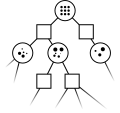
\includegraphics[width=\textwidth]{media/pomcpow_tree.pdf}
        \caption{POMCPOW Tree}
    \end{subfigure}
    \caption{Tree Structure Comparison. Each square is an action node, and each unfilled circle is an observation node. Each black dot corresponds to a state particle with the size representing its weight. In continuous observation spaces, the beliefs in a POMCP-DPW tree degenerate to a single particle, while POMCPOW maintains weighted particle mixture beliefs.}
    \label{fig:treecomp}
\end{figure}

\section{PFT-DPW}

Another algorithm that one might consider for solving continuous POMDPs online is MCTS-DPW on the equivalent belief MDP.
Since the Bayesian belief update is usually computationally intractable, a particle filter is used.
This new approach will be referred to as particle filter trees with double progressive widening (PFT-DPW).
It is shown in \cref{alg:pft}, where $G_\text{PF($m$)}(b,a)$ is a particle filter belief update performed with a simulated observation and $m$ state particles which approximates the belief MDP generative model.
The authors are not aware of any mention of this algorithm in prior literature, but it is very likely that MCTS with particle filters has been used before without double progressive widening under another name.

PFT-DPW is fundamentally different from POMCP and POMCPOW because it relies on simulating approximate belief trajectories instead of state trajectories.
This distinction also allows it to be applied to problems where the reward is a function of the belief rather than the state such as pure information-gathering problems \cite{dressel2017efficient,araya2010pomdp}.

The primary shortcoming of this algorithm is that the number of particles in the filter, $m$, must be chosen a-priori and is static throughout the tree.
Each time a new belief node is created, an $\mathcal{O}(m)$ particle filter update is performed.
If $m$ is too small, the beliefs may miss important states, but if $m$ is too large, constructing the tree is expensive.
Fortunately, the experiments in \cref{sec:experiments} show that it is often easy to choose $m$ in practice; for all the problems we studied, a value of $m=20$ resulted in good performance.


\begin{algorithm}
    \caption{PFT-DPW} \label{alg:pft}
    \begin{algorithmic}[1]
        \Procedure{Plan}{$b$}
            \For{$i \in 1:n$}
                \State $\Call{Simulate}{b, d_\text{max}}$
            \EndFor
            \State $\textbf{return } \underset{a}{\argmax}\, Q(ba)$
        \EndProcedure
        \Procedure {Simulate}{$b$, $d$}        
            \If{$d = 0$}
                \State \textbf{return} $0$
            \EndIf
            \State $a \gets \Call{ActionProgWiden}{b}$
            \If{$|C(ba)| \leq k_o N(ba)^{\alpha_o}$}
                \State $b',r \gets G_\text{PF($m$)}(b,a)$
                \State $C(ba) \gets C(ba) \cup \{(b',r)\}$
                \State $total \gets r + \gamma \Call{Rollout}{b', d-1}$
            \Else
                \State $b', r \gets \text{sample uniformly from } C(ba)$
                \State $total \gets r + \gamma \Call{Simulate}{b', d-1}$
            \EndIf
            \State $N(b) \gets N(b)+1$
            \State $N(ba) \gets N(ba)+1$
            \State $Q(ba) \gets Q(ba) + \frac{total - Q(ba)}{N(ba)}$
            \State \textbf{return} $total$
        \EndProcedure
    \end{algorithmic}
\end{algorithm}

\subsection{POMCPOW}

\begin{algorithm}[t]
    \caption{POMCPOW} \label{alg:pomcpow}
    \begin{algorithmic}[1]
        \Procedure {Simulate}{$s$, $h$, $d$}        
            \If{$d = 0$}
                \State \textbf{return} $0$
            \EndIf
            \State $a \gets \Call{ActionProgWiden}{h}$
            \State $s',o,r \gets G(s,a)$
            \If{$|C(ha)| \leq k_o N(ha)^{\alpha_o}$}
                \State $M(hao) \gets M(hao) + 1$
            \Else
                \State $o \gets \text{select } o \in C(ha) \text{ w.p. } \frac{M(hao)}{\sum_{o} M(hao)}$
            \EndIf
            \State $\text{append } s' \text{ to } B(hao)$ \label{lin:insert}
            \State $\text{append } \obsdist(o \mid s, a, s') \text{ to } W(hao)$ \label{lin:weight}
            \If{$o \notin C(ha)$} \Comment{new node}
                \State $C(ha) \gets C(ha) \cup \{o\}$
                \State $total \gets r + \gamma \Call{Rollout}{s', hao, d-1}$
            \Else
                \State $s' \gets \text{select } B(hao)[i] \text{ w.p. } \frac{W(hao)[i]}{\sum_{j=1}^m W(hao)[j]}$ \label{lin:sample}
                \State $r \gets R(s,a,s')$
                \State $total \gets r + \gamma \Call{Simulate}{s', hao, d-1}$
            \EndIf
            \State $N(h) \gets N(h)+1$
            \State $N(ha) \gets N(ha)+1$
            \State $Q(ha) \gets Q(ha) + \frac{total - Q(ha)}{N(ha)}$
            \State \textbf{return} $total$
        \EndProcedure
    \end{algorithmic}
\end{algorithm}


In order to address the suboptimality of POMCP-DPW, we now propose a new algorithm, POMCPOW, shown in \cref{alg:pomcpow}.
In this algorithm, the belief updates are weighted, but they also expand gradually as more simulations are added.
Furthermore, since the richness of the belief representation is related to the number of times the node is visited, beliefs that are more likely to be reached by the optimal policy have more particles.
At each step, the simulated state is inserted into the weighted particle collection that represents the belief (line~\ref{lin:insert}), and a new state is sampled from that belief (line~\ref{lin:sample}).
A simple illustration of the tree is shown in \Cref{fig:treecomp} to contrast with a POMCP-DPW tree.
Because the resampling in line~\ref{lin:sample} can be efficiently implemented with binary search, the computational complexity is $\mathcal{O}(n d \log(n))$.

\subsection{Discretization} \label{sec:discretization}

Discretization is perhaps the most straightforward way to deal with continuous observation spaces. The results in \cref{tab:experiments} show that this approach is only sometimes effective.
\Cref{fig:disc} shows the performance at different discretization granularities for the Light Dark and Sub Hunt problems.

Since the Light Dark domain has only a single observation dimension, it is easy to discretize.
In fact, POMCP with fine discretization outperforms POMCPOW.
However, discretization is only effective at certain granularities, and this is highly dependent on the solver and possibly hyperparameters.
In the Sub Hunt problem, with its high-dimensional observation, discretization is not effective at any granularity.
In Van Der Pol tag, both the action and observation spaces must be discretized.
Due to the high dimensionality of the observation space, similar to Sub Hunt, no discretization that resulted in good performance was found.

\begin{figure}[htb]
    \centering
    \begin{subfigure}{\linewidth}
        \centering
        \includegraphics[width=0.8\linewidth]{media/ld_discretization.pdf}
        \caption{Light Dark} \label{fig:lddisc}
    \end{subfigure}

    \begin{subfigure}{\linewidth}
        \centering
        \includegraphics[width=0.72\linewidth]{media/subhunt_discretization.pdf}
        \caption{Sub Hunt}
        \label{fig:shdisc}
    \end{subfigure}

    \caption{Discretization granularity studies} \label{fig:disc}
\end{figure}



\subsection{Observation Distribution Requirement}

It is important to note that, while POMCP, POMCP-DPW, and DESPOT only require a generative model of the problem,  both POMCPOW and PFT-DPW require a way to query the relative likelihood of different observations ($\obsdist$ in line~\ref{lin:weight}).
One may object that this will limit the application of POMCPOW to a small class of POMDPs, but we think it will be an effective tool in practice for two reasons.

First, this requirement is no more stringent than the requirement for a standard importance resampling particle filter, and such filters are used widely, at least in the field of robotics that the authors are most familiar with. 
Moreover, if the observation model is complex, an approximate model may be sufficient.

Second, given the implications of \cref{thm:qmdp}, it is difficult to imagine a tree-based decision-making algorithm or a robust belief updater that does not require some way of measuring whether a state belongs to a belief or history.
The observation model is a straightforward and standard way of specifying such a measure.
Finally, in practice, except for the simplest of problems, using POMCP or DESPOT to repeatedly observe and act in an environment already requires more than just a generative model.
For example, the authors of the original paper describing POMCP~\cite{silver2010pomcp} use heuristic particle reinvigoration in lieu of an observation model and importance sampling.

\section{Experiments} \label{sec:experiments}

Numerical simulation experiments were conducted to evaluate the performance of POMCPOW and PFT-DPW compared to other solvers. The open source code for the experiments is built on the POMDPs.jl framework \cite{egorov2017pomdps} and is hosted at \url{https://github.com/zsunberg/ContinuousPOMDPTreeSearchExperiments.jl}. In all experiments, the solvers were limited to \SI{1}{second} of computation time per step. Belief updates were accomplished with a particle filter independent of the planner, and no part of the tree was saved for re-use on subsequent steps. Hyperparameter values are shown in \cref{sec:hyper}.

\begin{table*}
    {\centering
        \caption{Experimental Results} \label{tab:experiments}


    \begin{tabular}{lrlrlrlrlrlrl}
        \toprule
            & Multilane \makebox[0pt][l]{(C, D, C)} & \\        
        \midrule
            POMCPOW & \result{0.3}{0.0}{77}{0.77} \\
PFT-DPW & \noresult{} \\
QMDP & \result{0.3}{0.0}{74}{0.74} \\
POMCP-DPW & \noresult{} \\
DESPOT & \result{0.4}{0.0}{90}{0.90} \\
POMCP\textsuperscript{D} & \noresult{} \\
DESPOT\textsuperscript{D} & \noresult{} \\

        \bottomrule
    \end{tabular}



%     \begin{tabular}{lrlrlrlrlrlrl}
%         \toprule
%             & Laser Tag \makebox[0pt][l]{(D, D, D)} & & Light Dark \makebox[0pt][l]{(D, D, C)} & & Sub Hunt \makebox[0pt][l]{(D, D, C)} & & VDP Tag \makebox[0pt][l]{(C, C, C)} & & Multilane \makebox[0pt][l]{(C, D, C)} & \\        
%         \midrule
%             POMCPOW & \result{-10.3}{0.2}{81}{0.81} & \result{56.1}{0.6}{76}{0.76} & \result{69.2}{1.3}{87}{0.87} & \result{29.3}{0.8}{95}{0.95} & \result{0.3}{0.0}{77}{0.77} \\
% PFT-DPW & \result{-11.1}{0.2}{74}{0.74} & \result{57.2}{0.5}{77}{0.77} & \result{77.4}{1.1}{97}{0.97} & \result{27.2}{0.8}{88}{0.88} & \noresult{} \\
% QMDP & \result{-10.5}{0.2}{79}{0.79} & \result{-6.4}{1.0}{14}{0.14} & \result{28.0}{1.3}{35}{0.35} & \noresult{} & \result{0.3}{0.0}{74}{0.74} \\
% POMCP-DPW & \result{-10.6}{0.2}{78}{0.78} & \result{-7.3}{1.0}{13}{0.13} & \result{28.3}{1.3}{35}{0.35} & \result{16.4}{1.0}{53}{0.53} & \noresult{} \\
% DESPOT & \result{-8.9}{0.2}{92}{0.92} & \result{-6.8}{1.0}{13}{0.13} & \result{26.8}{1.3}{34}{0.34} & \noresult{} & \result{0.4}{0.0}{90}{0.90} \\
% POMCP\textsuperscript{D} & \result{-14.1}{0.2}{49}{0.49} & \result{61.1}{0.4}{81}{0.81} & \result{28.0}{1.3}{35}{0.35} & \result{14.7}{0.9}{47}{0.47} & \noresult{} \\
% DESPOT\textsuperscript{D} & \noresult{} & \result{54.2}{1.1}{74}{0.74} & \result{27.4}{1.3}{34}{0.34} & \result{14.3}{1.0}{46}{0.46} & \noresult{} \\
% 
%         \bottomrule
%     \end{tabular}

    }
    \vspace{1mm}
    \footnotesize{The three C or D characters after the solver indicate whether the state, action, and observation spaces are continuous or discrete, respectively. For continuous problems, solvers with a superscript D were run on a version of the problem with discretized action and observation spaces, but they interacted with continuous simulations of the problem.}
\end{table*}

\subsection{Laser Tag}

The Laser Tag benchmark is taken directly from the work of \citet{somani2013despot} and included for the sake of calibration. DESPOT outperforms the other methods. The score for DESPOT differs slightly from that reported by \citet{somani2013despot} likely because of bounds implementation differences.
POMCP performs much better than reported by \citet{somani2013despot} because this implementation uses a state-based rollout policy.

\subsection{Light Dark}

In the Light Dark domain, the state is an integer, and the agent can choose how to move deterministically ($s' = s+a$) from the action space $\mathcal{A}=\{-10, -1, 0, 1, -10\}$. 
The goal is to reach the origin.
If action $0$ is taken at the origin, a reward of $100$ is given and the problem terminates; If action $0$ is taken at another location, a penalty of $-100$ is given.
There is a cost of $-1$ at each step before termination.
The agent receives a more accurate observation in the ``light'' region around $s=10$.
Specifically, observations are continuous ($\obsspace=\reals$) and normally distributed with standard deviation $\sigma=|s-10|$.

\Cref{tab:experiments} shows the mean reward from $1000$ simulations for each solver, and \cref{fig:ld} shows an example experiment.
The optimal strategy involves moving toward the light region and localizing before proceeding to the origin. 
QMDP and solvers predicted to behave like QMDP attempt to move directly to the origin, while POMCPOW and PFT-DPW perform better.
In this one-dimensional case, discretization allows POMCP to outperform all other methods and DESPOT to perform well, but in subsequent problems where the observation space has more dimensions, discretization does not provide the same performance improvement (see \cref{sec:discretization}).

\begin{figure}[htb]
    \centering
    % \input{ld_fig.pgf}
    \includegraphics[width=\columnwidth]{media/ld_fig.pdf}
    \caption{Example trajectories in the Light Dark domain. POMCPOW travels to the light region and accurately localizes before moving to the goal. POMCP-DPW displays QMDP-like behavior: it is unable to localize well enough to take action \num{0} with confidence. The belief particles far away from \num{0} in the POMCP-DPW plot are due to particle reinvigoration that makes the filter more robust.}
    \label{fig:ld}
\end{figure}

\subsection{Sub Hunt}

In the Sub Hunt domain, the agent is a submarine attempting to track and destroy an enemy sub.
The state and action spaces are discrete so that QMDP can be used to solve the problem for comparison.
The agent and the target each occupy a cell of a 20 by 20 grid. The target is either aware or unaware of the agent and seeks to reach a particular edge of the grid unknown to the agent ($\mathcal{S} = \{1,..,20\}^4 \times \{\text{aware}, \text{unaware}\} \times \{N,S,E,W\}$).
The target stochastically moves either two steps towards the goal or one step forward and one to the side.
The agent has six actions, move three steps north, south, east, or west, engage the other submarine, or ping with active sonar.
If the agent chooses to engage and the target is unaware and within a range of 2, a hit with reward 100 is scored; The problem ends when a hit is scored or the target reaches its goal edge.

An observation consists of 8 sonar returns ($\obsspace = \reals^8$) at equally-spaced angles that give a normally distributed estimate ($\sigma=0.5$) of the range to the target if the target is within that beam and a measurement with higher variance if it is not.
The range of the sensors depends on whether the agent decides to use active sonar.
If the agent does not use active sonar it can only detect the other submarine within a radius of 3, but pinging with active sonar will detect at any range.
However, active sonar alerts the target to the presence of the agent, and when the target is aware, the hit probability when engaging drops to $60\%$.

\Cref{tab:experiments} shows the mean reward for $1000$ simulations for each solver.
The optimal strategy includes using the active sonar, but previous approaches have difficulty determining this because of the reduced engagement success rate.
The PFT-DPW approach has the best score, followed closely by POMCPOW.
All other solvers have similar performance to QMDP.


\subsection{Van Der Pol Tag} \label{sec:vdptag}

\begin{figure}[bth]
    \centering
    \begin{minipage}{0.5\linewidth}
        \centering
        \includegraphics[width=0.8\linewidth]{media/vdp_quiver.pdf}
    \end{minipage}
    \hfill
    \begin{minipage}[c]{0.45\linewidth}
        \caption{Van Der Pol tag problem. The arrows show the target differential equation, and the thick black lines represent the barriers.}
        \label{fig:vdp}
    \end{minipage}
\end{figure}


The final experimental problem is called Van Der Pol tag and has continuous state, action, and observation spaces.
In this problem an agent moves through 2D space to try to tag a target ($\mathcal{S}=\reals^4$) that has a random unknown initial position in $[-4, 4]\times[-4,4]$.
The agent always travels at the same speed, but chooses a direction of travel and whether to take an accurate observation ($\mathcal{A} = [0, 2\pi)\times\{0,1\}$).
The observation again consists of 8 beams ($\obsspace=\reals^8$) that give measurements to the target.
Normally, these measurements are too noisy to be useful ($\sigma=5$), but, if the agent chooses an accurate measurement with a cost of \num{5}, the observation has low noise ($\sigma=0.1$).
The agent is blocked if it comes into contact with one of the barriers that stretch from \num{0.2} to \num{3.0} in each of the cardinal directions (see \cref{fig:vdp}), while the target can move freely through.
There is a cost of \num{1} for each step, and a reward of \num{100} for tagging the target (being within a distance of \num{0.1}).


The target moves following a two dimensional form of the Van Der Pol oscillation defined by the differential equations%
\begin{equation}
    \dot{x} = \mu \left( x - \frac{x^3}{3} -y \right) \quad \text{ and }\quad \dot{y} = \frac{1}{\mu}x\text{,} \nonumber
\end{equation}
where $\mu=2$.
Gaussian noise ($\sigma=0.05$) is added to the position at the end of each step.
Runge-Kutta fourth order integration is used to propagate the state.

This problem has several challenging features that might be faced in real-world applications.
First, the state transitions are more computationally expensive because of the numerical integration.
Second, the continuous state space and obstacles make it difficult to construct a good heuristic rollout policy, so random rollouts are used.
\Cref{tab:experiments} shows the mean reward for $1000$ simulations of this problem for each solver.
Since a POMCPOW iteration requires less computation than a PFT-DPW iteration, POMCPOW simulates more random rollouts and thus performs slightly better.


\subsection{Hyperparameters} \label{sec:hyper}

\begin{table}[t]
    {\centering
\caption{Hyperparameters used in experiments} \label{tab:hyper}

\begin{center}
\begin{tabular}{lrrrr}
    \toprule
                & Laser Tag     & Light Dark    & Sub Hunt      & VDP Tag \\
    \midrule
    \multicolumn{3}{l}{POMCPOW} \\
    \midrule
    $c$         & \num{26.0}    & \num{90.0}    & \num{17.0}    & \num{110.0} \\
    $k_a$       & --            & --            & --            & \num{30.0}  \\
    $\alpha_a$  & --            & --            & --            & \num{1/30}  \\
    $k_o$       & \num{4.0}     & \num{5.0}     & \num{6.0}     & \num{5.0}   \\
    $\alpha_o$  & \num{1/35}    & \num{1/15}    & \num{1/100}   & \num{1/100} \\
    \midrule
    \multicolumn{3}{l}{PFT-DPW} \\
    \midrule
    $m$         & \num{20}      & \num{20}      & \num{20}      & \num{20}    \\
    $c$         & \num{26.0}    & \num{100.0}   & \num{100.0}   & \num{70.0}  \\
    $k_a$       & --            & --            & --            & \num{20.0}  \\
    $\alpha_a$  & --            & --            & --            & \num{1/25}  \\
    $k_o$       & \num{4.0}     & \num{4.0}     & \num{2.0}     & \num{8.0}   \\
    $\alpha_o$  & \num{1/35}    & \num{1/10}    & \num{1/10}    & \num{1/85}  \\
    \midrule

\end{tabular}
\end{center}
    }
    \vspace{1mm}

    \footnotesize{For problems with discrete actions, all actions are considered and $k_a$ and $\alpha_a$ are not needed.}
\end{table}

Hyperparameters for POMCPOW and PFT-DPW were chosen using the cross entropy method \cite{mannor2003cross}, but exact tuning was not a high priority and some parameters were re-used across solvers so the parameters may not be perfectly optimized.
The values used in the experiments are shown in \cref{tab:hyper}. 
There are not enough experiments to draw broad conclusions about the hyperparameters, but it appears that performance is most sensitive to the exploration constant, $c$.

The values for the observation widening parameters, $k_o$ and $\alpha_o$, were similar for all the problems in this work.
A small $\alpha_o$ essentially limits the number of observations to a static number $k_o$, resulting in behavior reminiscent of sparse UCT \cite{browne2012survey}, preventing unnecessary widening and allowing the tree to grow deep.
This seems to work well in practice with the branching factor ($k_o$) set to values between \num{2} and \num{8}, and suggests that it may be sufficient to limit the number of children to a fixed number rather than do progressive widening in a real implementation.



\chapter{POMDPs.jl: A Framework for Sequential Decision Making under Uncertainty} \label{chap:pomdpsjl}

Since exact optimal solutions to POMDPs can rarely be attained, most research into solving realistic problems involves empirical comparison between solution techniques.
Sharing solver software between researchers can greatly improve speed and quality of this work.
Moreover, a consistent and concise framework for representing problems and demonstrating solution techniques is invaluable for POMDP education.
This chapter describes the POMDPs.jl software package created by the Stanford Intelligent Systems Lab (SISL) to make state-of-the-art POMDP solution methods easily accessible to students, researchers, and engineers.
All of the research in \cref{chap:multilane,chap:pomcpow} was conducted using this framework.

The POMDPs.jl package itself is implementation-free, and contains only the interface, however the JuliaPOMDP organization maintains several other packages that provide tools and concrete implementations. For example, the POMDPToolbox package contains a variety of useful tools for representing common distributions, beliefs, policies, etc. and the POMDPModels package contains some simple problem implementations.

\section{Challenges for POMDP-solving software}

A successful POMDP software framework must have, at a minimum, the following attributes: speed, flexibility, and ease of use. Achieving all of these attributes simultaneously is a major challenge.

\subsection{Speed}

Since POMDPs are difficult to solve~\cite{papadimitriou1987complexity}, any computational slowdown such as unnecessary memory allocation or runtime type inference significantly reduces the maximum problem size that the framework can handle.
For this reason, POMDP algorithms must be compiled to efficient processor instructions with low overhead.

\subsection{Flexibility}

The set of problems that can be represented as a POMDP is extremely large and there are many possible characteristics that such problems might have.
A good POMDP software framework should try to accommodate as much of this set as possible.
A few of the most important model characteristics to support are outlined below.

\subsubsection{Partial and full observability}

When studying a POMDP problem, it is almost always important to analyze the underlying fully-observable problem.
Thus, a good POMDP framework should have first-class support for MDPs in addition to POMDPs.

\subsubsection{Continuous and discrete problems}

Some POMDPs have a finite number of states, actions, and observations, i.e. $|\sspace| < \infty$, $|\aspace| < \infty$, and $|\ospace| < \infty$.
However, many real world problems, notably robotics problems, are naturally formulated in spaces with uncountably infinite cardinality, e.g. $\sspace = \reals$, $\aspace = \reals$, and $\ospace = \reals$, multi-dimensional vector spaces, e.g. $\sspace = \reals^6$, or hybrid continuous-discrete spaces.
This means that the framework must not be constrained to use integers for state representation, but should be capable of using a range of structures including floating point numbers and arrays.

\subsubsection{Explicit vs generative model representation}

Some POMDP and MDP solution techniques use the explicit probability distributions $\tdist$ and $\odist$ to solve problems.
Thus, a successful framework must include a way to explicitly specify $\tdist$ and $\odist$.
On the other hand, explicitly specifying $\tdist$ and $\odist$ for many realistic problems is exceedingly difficult and tedious, and specifying a generative model is the only practical way to encode the problem.
Thus, a successful framework must also include generative model support.

\subsubsection{Online and offline solvers}

While some POMDP solution techniques seek exact offline solutions to small problems, many larger problems can only be practically solved online.
Thus a good POMDP framework must have first class support for solving offline and efficiently executing a policy online or executing a planner that does significant computation online.

\subsubsection{Policy representation}

The policies that different solution techniques yield can take a variety of forms.
Exact solution techniques typically attempt to find alpha vectors that encode an optimal policy \cite{kaelbling1998planning,kurniawati2008sarsop}, whereas others use finite state machines \cite{bai2010mcvi}.
Newer methods may use neural networks \cite{karkus2017qmdp} or other structures to store policies, so a successful framework must provide a flexible way to represent all of these structures.

\subsection{Ease of Use}

In addition to being flexible and performant, the framework must be easy to use.
It is possible to make a framework that is performant and flexible but so complex that it will not be adopted or will cause much time to be wasted in understanding and implementation.
For the framework to be considered a success, it must be adopted by the community and serve as an enabler rather than a hindrance to research.

\section{Previous frameworks}

A number of frameworks exist for solving sequential decision problems.
However, most frameworks are written from a reinforcement learning perspective and hence only support either fully observable problems or problems where the state is fully observable, or environments that can generate observations but do not provide access to the Markov state structure of the problem.
Examples from this class are BURLAP~\cite{diuk2008object}, RLPy~\cite{geramifard2015rlpy}, and rllab~\cite{duan2016benchmarking}.
The most closely related frameworks to POMDPs.jl are APPL~\citep{appl}, AI-Toolbox~\citep{aitoolbox}, and ZMDP~\citep{zmdp} in that they explicitly represent the state and partial observability.
\todo{Check if BURLAP and ai toolbox actually do what I say}

APPL is the most widely used and up to date of these POMDP frameworks.
It is written efficiently in C++ and is excellent from a speed perspective.
However, it has several shortcomings in terms of flexibility and ease of use.
First, though all of the solvers in APPL support the POMDPX file format for discrete, explicit problem definitions, flexibility is limited because there is not a unified interface for defining generative models or continuous explicit models.
Second, prototyping problems and solvers in this framework is relatively time consuming and complex, making it difficult to use.
Specifically, the POMDPX file format is based on XML and is difficult for humans to write directly, so, in most cases, custom scripts must be written to create the files, and solvers and generative models written in C++ have higher development time costs than those written in a higher level language.

\todo{Check to make sure there is not a unified distribution}
\todo{Get quote from APPL}

Though much research progress has been made with these frameworks, POMDPs.jl offers several significant improvements.

\section{Architecture}

POMDPs.jl is designed to facilitate communication between different people performing three actions: defining problems, writing solver software, and running simulation experiments.
The same person will often operate in two or even all three of these roles, but will nearly always bring in some tools written by others.

The framework derives its solutions to the challenges outlined above primarily through the use of the Julia language itself \cite{bezanson2017julia}.
Julia is just-in-time compiled using the state-of-the art LLVM compiler framework, giving it speed comparable to traditional compiled languages such as C and C++.
However, unlike other compiled languages, it has many features that make numerical software development easier and faster.
For example, like Python, it is dynamically typed, has a powerful and flexible type system, and uses a modern, convenient syntax with features like list comprehensions, and, like Matlab, it has built-in efficient multidimensional arrays and linear algebra.
The makes meeting the flexibility and ease-of-use goals much easier.

\todo{cite LLVM}
\todo{Make sure Julia is dynamically typed}

This section describes some of the concepts used in the framework before outlining the interface itself.

\subsection{Concepts} \label{sec:concepts}

To fulfill each of the roles mentioned above, a programmer implements one or more classes that concretely represent concepts used to describe POMDP solving.
The problem writer creates a concrete subtype of the \texttt{POMDP} or \texttt{MDP} abstract classes to represent a problem, the simulator writer creates a \texttt{Simulator} type to run simulations, and the solver writer creates a \texttt{Solver} subtype to run computations offline, and a \texttt{Policy} subtype to execute a policy online.

In POMDPs.jl the term ``Belief'' is used to mean any structure that encodes the information needed to execute the policy.
For instance, if the policy is encoded as a set of alpha vectors, the belief takes its usual meaning as an explicit probability distribution over the states; for an online solver like POMCP, it must generate states for the tree search; and for a finite-state-machine policy like the one created by MCVI, it is simply the id of the current node.
An \texttt{Updater} in POMDPs.jl is an object that defines how information from new observations is integrated into the belief.
For example, if the belief is a probability distribution, the updater would apply Bayes rule or an approximation.
Since the belief is often closely related to the policy, the solver writer will often implement the \texttt{Updater}, however generic updaters such as particle filters are also available.
\Cref{fig:concepts} shows the three role concepts and some of the associated abstract types and interface functions.

\begin{figure}[htpb]
    \centering
    \includegraphics[width=0.8\linewidth]{media/arch.pdf}
    \caption[POMDPs.jl concepts]{POMDPs.jl concepts. POMDPs.jl facilitates communication between people in three roles. The abstract types are shown beside each node and some of the interface functions are shown between the nodes. The arrows indicate which roles use code from which other roles.}
    \label{fig:concepts}
\end{figure}

\subsection{Interfaces}

The behavior of POMDPs.jl objects is defined by implementing methods of interface functions.
Implementing interface functions serves as an alternative to writing configuration files such as POMDPX files or specifications in purpose-built languages like RDDL~\cite{sanner2010rddl} in previous frameworks.
For example the problem writer may implement a method of the \texttt{reward} function that returns the reward given a problem instance, state and action.
Julia will call the correct \texttt{reward} method for the problem type based on its multiple dispatch system \cite{bezanson2017julia}.
Similarly, an \texttt{Updater} should have a corresponding \texttt{update} method that returns a new belief given an updater object, previous belief, action, and observation.
The complete interface is not listed here, but is available in the online documentation.

In POMDPs.jl, states, actions, observations, beliefs, and distributions can be represented by objects of any type as long as the appropriate interface methods are implemented.
This provides the flexibility needed to represent continuous or discrete problems.
Packages in the Julia ecosystem provide convenient and efficient types for common state representations, such as small fixed-size vectors.

One flexibility goal that has not been met by previous frameworks is support of both generative and explicit problem definitions.
For example, in APPL, all solvers can handle POMDPX problem specification for explicit definitions, but the MCVI and DESPOT solvers use different interfaces for generative problems, and there is no way to represent continuous problems explicitly.
POMDPs.jl overcomes this challenge by exposing both an explicit interface and generative interface that can be mixed.
If the necessary parts of the explicit interface are implemented for a problem, POMDPs.jl will automatically provide the generative interface functions for the problem.
The interface relationships are illustrated in \cref{fig:interfaces}.
Implementations of all of the interface functions are not strictly required; if the minimum set of functions used by a solver or simulator are implemented for a problem, then that solver or simulator will work with that problem.

\begin{figure}[htpb]
    \centering
    \includegraphics[width=0.8\linewidth]{media/interfaces.pdf}
    \caption{POMDPs.jl interfaces}
    \label{fig:interfaces}
\end{figure}

Because of the interface's flexibility, expressing which interface functions a problem-writer should implement, giving helpful error messages, and even checking whether a sufficient portion of the interface has been implemented is a complex challenge.
For example, suppose a user intends to implement a complex problem that cannot easily be expressed with an explicit definition and intends to use a solver that only requires functions from the generative interface.
If POMDPs.jl advises this user to implement functions from the explicit interface, he or she will conclude that expressing the problem is difficult or impossible.
This complexity drove the development of an interface and framework for dynamically specifying requirements and dependencies and generating helpful reports for users.
In this requirements framework, built with Julia's powerful metaprogramming features, solver and simulator writers declare the requirements for their algorithm, which may be based on solver options, and problem writers can check which of the requirements have been satisfied by their problem implementation.
Examples of the output of this system are shown in \cref{fig:requirements}.

\begin{figure}[htpb]
    \centering
    \begin{subfigure}[b]{0.48\textwidth}
    \begin{center}
        \includegraphics[width=\textwidth]{media/requirements_info_new.png}
    \end{center}
    \caption{New problem with no methods}
    \end{subfigure}
    \hfill
    \begin{subfigure}[b]{0.48\textwidth}
    \begin{center}
        \includegraphics[width=\textwidth]{media/requirements_info_gw.png}
    \end{center}
    \caption{Fully implemented problem}
    \end{subfigure}
     
    \caption[POMDPs.jl requirements example]{POMDPs.jl requirements example output for the value iteration solver}
    \label{fig:requirements}
\end{figure}

\section{Examples}

This section presents simple examples illustrating implementations of the concepts in~\cref{sec:concepts}, namely the problem, the solver, and the experiment. 

\lstset{escapechar=@,style=customjulia}

\subsection{Problem}

The problem defines the MDP or POMDP model to be solved.
%The user decides how to define the model components.
For this example, consider the Tiger POMDP example of \citet{kaelbling1998planning}.

\begin{lstlisting}
 struct TigerPOMDP <: POMDP{Symbol, Symbol, Symbol}
     p_correct::Float64 # probability of hearing the tiger correctly
     discount::Float64  # discount factor
 end
\end{lstlisting}
%
The \code{TigerPOMDP} type is a subtype of the abstract {\small\ttfamily POMDP} type 
The three parameters of \code{POMDP} denote the types used to represent the states, actions, and observations.
These can be any types including built-in Julia types or special-purpose user defined types.
Here \code{Symbol}s (interned strings) are used for the sake of readability, but \code{Bool}s, \code{Int}s, or a custom enumeration could also easily be used.
% In this case, since the tiger is behind one of two doors, the state is represented by the native \code{Bool}.
% Similarly, since there are three actions, an \code{Int} is used to represent each, and a \code{Bool} represents each observation.
% The constants make the code easier to read.
 
The problem behavior is defined by implementing new methods of the functions in the POMDPs.jl interface.
For example, the function below returns the observation distribution for the Tiger POMDP given an action and state.

\begin{lstlisting}
 function POMDPs.observation(pomdp::TigerPOMDP, a::Symbol, sp::Symbol)
     pc = pomdp.p_correctly
     if a == :listen
         if sp == :tiger_left
             p = pomdp.p_correct
         else
             p = 1.0 - pomdp.p_correct
         end
     else
         p = 0.5
     end
     return SparseCat([:tiger_left, :tiger_right], [p, 1.0-p])
 end
\end{lstlisting}

The \code{SparseCat} object returned by this method is provided by the POMDPToolbox package, represents a (potentially sparse) categorical distribution over a list of objects.
Other code can randomly sample from the \code{SparseCat} distribution, query its probability distribution, and efficiently iterate over the members with nonzero probability.

Since the state in the Tiger POMDP never changes, the transition dynamics can be expressed concisely as
\begin{lstlisting}
 function POMDPs.transition(pomdp::TigerPOMDP, s::Symbol, a::Symbol)
     if a == :listen
         return SparseCat([s], [1.0]) 
     else # a looking action - the problem finishes
         return SparseCat([:done], [1.0])
     end
 end
\end{lstlisting}

The entire problem definition contains several more methods, including \code{reward}, \code{actions}, \code{discount}, \code{isterminal}, etc.

\subsection{Solver} 

A solver implementation requires between one and three type definitions: a \code{Solver} that contains the parameters that define solver behavior, often a \code{Policy} that defines a mapping from beliefs to actions, and sometimes an \code{Updater} if the belief is closely linked to how the policy functions.
Some example code for the QMDP~\citep{littman1995} solution method is shown below.

QMDP works by running value iteration on the fully observable MDP at the core.
In the \code{solve} function, partially listed below, the POMDPs.jl functions which will have methods for the particular POMDP being solved are called.
Once value iteration has completed, an \code{AlphaVectorPolicy} from POMDPToolbox.jl is returned.
The ellipses indicate code that has been left out for the sake of brevity.

\begin{lstlisting}
 function POMDPs.solve(solver::QMDPSolver, pomdp::POMDP)
     ...
     for i in 1:solver.max_iterations
         ...
         for (istate,s) in enumerate(states)
             if isterminal(mdp, s)
                 util[istate] = 0.0
                 ...
             else
                 ...
                 for a in iterator(actions(pomdp, s))
                     dist = transition(mdp, s, a)
                     u = 0.0
                     for (sp, p) in weighted_iterator(dist)
                         r = reward(pomdp, s, a, sp)
                         isp = state_index(pomdp, sp)
                         u += p * (r + discount(pomdp) * util[isp])
                 ...
     return AlphaVectorPolicy(qvalues)
 end
\end{lstlisting}

\subsection{Simulator}

POMDP Solution algorithms are typically evaluated by running Monte Carlo simulations.
A \code{Simulator} calls POMDPs.jl functions defined for the solver and the problem to run a simulation and return the desired statistics from that simulation.
For example, the experimenter might create a simulator type, {\ttfamily Sim}, and a corresponding {\ttfamily simulate} function (an important part of the main loop is shown below).
\begin{lstlisting}
 function simulate(sim::Sim, pomdp::POMDP, policy::Policy, updater::Updater, initial_dist)
    ...
    for t in 1:sim.max_steps
        a = action(policy, b)
        sp = rand(sim.rng, transition(pomdp, s, a))
        r_total += discount(pomdp)^t*reward(pomdp, s, a, sp)
        o = rand(sim.rng, observation(pomdp, s, a, sp))
        b = update(updater, b, a, o)
        ...
\end{lstlisting}

With the examples above and the appropriate additional methods defined, a simulation can then be run as follows: 
\begin{lstlisting}
 pomdp = TigerPOMDP()           # initialize the tiger problem
 solver = QMDPSolver()          # initialize QMDP solver
 policy = solve(solver, pomdp)  # compute a policy
 r = simulate(Sim(), pomdp, policy, updater(policy), DiscreteBelief(2))
\end{lstlisting}

\section{Summary}

By using the leverage of the Julia programming language, POMDPs.jl provides an unprecedented level of flexibility for expressing and solving POMDPs. It is being used by other researchers to investigate topics as diverse as GPS jammer detection by drones and cancer screening recommendations, along with numerous student projects for a course taught at Stanford.

\todo{See if I can cite some things}

However, there is still much work to be done.
First, for the simplest examples, POMDPs.jl is a rather clumsy interface in that it requires methods to be implemented to define behavior.
Some of the best interfaces for expressing mathematical optimization problems, such as JuMP~\cite{dunning2017jump} and CVX~\cite{grant2014cvx}, have concise, declarative interfaces that can express problems in a few lines of code and be easily interpreted by looking at one page for a short time.
The POMDP domain is much more diverse and complex than the optimization domains addressed by these packages, but a concise declarative interface that can represent a subset of POMDPs would be very helpful in the education mission of POMDPs.jl.

Second, many of the solvers are far from achieving the full performance potential of the algorithms that they implement.
Since most modern hardware performance increases are due to parallelism rather than single-process speed increases, one of the most important factors in speeding up solver code is parallel implementation.
Though Julia has built-in tools for parallel processing, only a few of the solvers have parallel capabilities because many of the important factors in efficient parallelism, such as proper cache usage, have many pitfalls.
An investment of effort into parallelizing solver code would make the POMDPs.jl ecosystem much more useful.

\chapter{Summary and Future Work}

In order to realize benefits of autonomous transportation, the control systems of autonomous vehicles must be safe.
However, if this safety brings too great a sacrifice in efficiency, the vehicles will not be adopted as widely or be as useful.
This thesis investigated approaches for improving safety while sacrificing minimal efficiency, specifically by proposing better methods for handling the uncertainty inherent in the environment autonomous vehicles operate in.
In addition, the thesis proposed improved algorithms for solving the optimization problems that arise from vehicle control problems
Finally, it described the software framework created to make education and research collaboration in this area easier.
The remainder of this chapter reviews the specific contributions of this thesis and outlines potential future research directions.

\section{Contributions and Summary}

The first contribution (\cref{chap:uav}) is an investigation into the \textbf{combination of trusted resolution logic and optimization} for UAV collision avoidance.
Simple TRL has the advantage that guarantees about its operation are relatively easy to certify.
However, a comparison between simple TRL alone and MDP optimization shows that there is a price in terms of both safety and efficiency accrued for using the TRL.
To reduce this price, two methods for combining the approaches are investigated.
The first is to use an MDP policy to dynamically adjust the parameters of the TRL that govern its conservativeness.
The second is to use the TRL as a constraint on the actions that the MDP policy can choose.
Simulation experiments show that the second approach is superior.

The second contribution (\cref{chap:multilane}) is a \textbf{study of uncertainty modeling in decision making for autonomous highway lane changing}.
This chapter considered approximate POMDP solutions where the internal states of other drivers are explicitly modeled as a hidden part of the Markov state.
The POMDP solutions are compared with approximate MDP solutions, both assuming full knowledge of the internal state and conservatively modeling state uncertainty as outcome uncertainty.
\textbf{The advantage of POMDP solutions over MDP solutions is clear} in all of the tests, but the relative effectiveness of different POMDP approximations depends greatly on the correlation of the different internal state parameters.
Simulation tests show that when the parameters are highly correlated, since it is easier to estimate the hidden states, even greatly simplified POMDP approximations can achieve performance near the upper bound established by an omnipotent planner.
On the other hand, when there is little or no correlation, POMDP solution methods that include more of the uncertainty in the solution process perform significantly better.
Experiments also characterize the robustness of the algorithms with respect to the parameter distribution.

The third contribution (\cref{chap:pomcpow}) is a pair of \textbf{improved algorithms for solving POMDPs online}.
Previous leading online algorithms have focused on solving discrete problems, and are unable to solve problems with continuous action and observation spaces.
Hence, new algorithms for the continuous domains encountered in the real world are needed.
The first part of this contribution (\cref{sec:pomcpdpw}) is proving that \textbf{a naive application of double progressive widening to the POMCP algorithm will result in suboptimal behavior}.
In particular, in a continuous observation space, it will converge to the QMDP solution because each belief node will degenerate to a single state particle (\cref{thm:qmdp}).
In fact, numerical experiments confirm that all leading online solvers exhibit this behavior.

In response to this suboptimality, two new algorithms are proposed (\cref{sec:pftdpw,sec:pomcpow}).
The first, PFT-DPW, solves an approximation of the belief MDP, while the second, \textbf{POMCPOW}, is an extension of POMCP with double progressive widening and weighted particle filtering.
Numerical experiments (\cref{sec:experiments}) show that these algorithms are able to break the QMDP barrier and hence exhibit performance that is qualitatively superior to previous algorithms.
POMCPOW and PFT-DPW perform similarly on most problems, but on the most realistic problem, a version of the autonomous driving problem from~\cref{chap:multilane}, POMCPOW outperforms PFT-DPW.

The final contribution (\cref{chap:pomdpsjl}) is a software framework, \textbf{POMDPs.jl}, which provides an interface for expressing MDPs and POMDPs and tools for developing and testing solvers.
This framework is unprecedented in its flexibility.
It can represent discrete and continuous MDPs defined by both explicit probability distributions and simulators that provide generative models.
The Julia language also gives solvers written to use the framework speed comparable to previous C++ implementations.

\section{Future Work}

There are many promising directions for future work to proceed from the results presented in this thesis.
The discussion portion of each chapter gives short-term specific extensions to the individual research efforts described therein.
This section gives a broader overview.

The first line of future work involves \textbf{safety constraints}.
Interaction of safety constraints with sequential optimization is explored in \cref{chap:uav} and such constraints are used in \cref{chap:multilane}.
However, the actual constraints used there are very simple.
In real problems, these constraints will need to be more complex, consisting of, for example, linear temporal logic rules~\cite{sadigh2016safe} or results from reachability analysis~\cite{chen2015exact}.
Combining approximate POMDP solutions with these advanced safety constraints to field a reliable system still requires much research.

The second line is focused on \textbf{modeling}. \Cref{chap:uav,chap:multilane} evaluate their findings based on simplistic models of other vehicles.
To solidify the conclusions of this thesis, better data-driven models of human drivers and pilots must be created.
Indeed, significant work has already been done in this area~\cite{schmerling2018multimodal,bhattacharyya2018multi}. 
However, these models are limited in scope, primarily because of the limited data available.
In order to be able to test in more diverse scenarios, more data will need to be collected from the real world, and models that are more data-efficient developed.
Moreover, current planning algorithms will not work efficiently with certain models.
A particular example is that recurrent neural networks with latent states the represent beliefs over internal states~\cite{schmerling2018multimodal} will not work with the POMDP algorithms used in this thesis.
Thus, new algorithms must be developed to work with the new models.

The third direction is continuing the development of better \textbf{POMDP algorithms}.
While the algorithms proposed in \cref{chap:pomcpow} demonstrate better performance than previous algorithms, the shortcomings of this family of algorithms are also apparent.
In particular, algorithms based on MCTS-DPW have many tuning parameters that must be chosen via unreliable hand tuning or time consuming optimization.
In addition, the proof of consistency for MCTS-DPW~\cite{auger2013continuous} is rather tedious, which is one of the reasons that an analytical proof for the optimality of POMCPOW was not attempted for this thesis.
Moreover, the trees produced by these algorithms tend to be shallow, reducing the effective planning horizon.
As seen in the experimental results for the multilane model in \cref{tab:experiments}, DESPOT is able to perform better on more realistic problems because it builds deeper trees and explores based on bounds rather than upper confidence estimates.
DESPOT's fixed number of scenarios may also make analysis easier.
Given these advantages, the particle filter weighting approaches used in PFT-DPW and POMCPOW should be applied to more advance algorithms like DESPOT to enable them to explore in continuous observation spaces.
Furthermore, all of the algorithms discussed in this thesis use a single execution thread. In order to take advantage of modern computing hardware, online parallel algorithms for solving POMDPs must be investigated.

Finally, the problem of controlling autonomous vehicles in continuous, partially observable domains has by no means been solved.
One reason is the weakness of decision-making \textbf{algorithms for continuous spaces} that can handle uncertainty and irregularity.
This thesis focused on continuous state and observation spaces, but the action space is arguably the most difficult context for continuity.
Some research has begun to address this~\cite{seiler2015online,wang2018online}, but these algorithms use only derivative-free optimization techniques that may not scale to high dimensional problems.
In many continuous problems, if history $h_1$ consists of actions and observations near the actions and observations of history $h_2$, the value at $h_1$ will be very close to the value at $h_2$.
This information is not exploited in any of the online solvers discussed in this thesis.
Although some work has been done to use this information in MCTS~\cite{xiao2018memory}, new algorithms that use ideas from optimal control, model predictive control, and motion planning may be much better suited for continuous problems.


% and the end material

\appendix
% 
\chapter{Proof of Theorem 1} \label{sec:proof}

A version of Monte Carlo tree search with double progressive widening has been proven to converge to the optimal value function on fully observable MDPs by \citet{auger2013continuous}.
We use this proof to show that POMCP-DPW converges to the QMDP solution.

First we establish some preliminary definitions taken directly from \citet{auger2013continuous}.

\begin{definition}[Regularity Hypothesis]
    The \emph{Regularity hypothesis} is the assumption that for any $\Delta > 0$, there is a non zero probability to sample an action that is optimal with precision $\Delta$. More precisely, there is a $\theta > 0$ and a $p > 1$ (which remain the same during the whole simulation) such that for all $\Delta > 0$, 
\begin{align}
    Q(ha) \geq Q^*(h)-\Delta \text{ with probability at least } \min(1, \theta \Delta^p)\text{.}
\end{align}
\end{definition}

\begin{definition}[Exponentially sure in $n$]
    We say that some property depending on an integer $n$ is exponentially sure in $n$ if there exists positive constants $C$, $h$, and $\eta$ such that the probability that the property holds is at least $$1-C \exp(-hn^\eta)\text{.}$$
\end{definition}

In order for the proof from \citet{auger2013continuous} to apply, the following four minor modifications to the POMCP-DPW algorithm must be made: 

\begin{enumerate}
    \item Instead of the usual logarithmic exploration, use \emph{polynomial exploration}, that is, select actions based on the criterion
    \begin{equation}
        Q(ha) + \sqrt{\frac{N(h)^{e_d}}{N(ha)}}\text{,}
    \end{equation}
    as opposed to the traditional criterion
    \begin{equation}
        Q(ha) + c \sqrt{\frac{\log N(h)}{N(ha)}}\text{,}
    \end{equation}
    and create a new node for progressive widening when $\lfloor N^\alpha \rfloor > \lfloor (N-1)^\alpha \rfloor$ rather than when the number of children exceeds $k N^\alpha$.

    \item Instead of performing rollout simulations, keep creating new single-child nodes until the maximum depth is reached.

    \item In line~\ref{lin:selecto}, instead of selecting an observation randomly, select the observation that has been visited least proportionally to how many times it has been generated.

    \item Use the depth-dependent coefficient values in Table 1 from \citet{auger2013continuous} instead of choosing static values.
\end{enumerate}

This version of the algorithm will be referred to as ``modified POMCP-DPW''. The algorithm with these changes is listed in \Cref{alg:mpomcpdpw}.

\begin{algorithm}[htb]
    \caption{Modified POMCP-DPW} \label{alg:mpomcpdpw}
    \begin{algorithmic}[1]
        \Procedure{Plan}{$b$}
            \For{$i \in 1:n$}
                \State $s \gets \text{sample from }b$ \label{lin:msample}
                \State $\Call{Simulate}{s, b, d_\text{max}}$
            \EndFor
            \State $\textbf{return } \underset{a}{\argmax}\, Q(ba)$
        \EndProcedure

        \Procedure {ActionProgWiden}{$h$}
            \If{$\lfloor N(h)^{\alpha_{a,d}} \rfloor > \lfloor (N(h)-1)^{\alpha_{a,d}} \rfloor$}
                \State $a \gets \Call{NextAction}{h}$
                \State $C(h) \gets C(h) \cup \{a\}$
            \EndIf
            \State $\textbf{return } \underset{a \in C(h)}{\argmax}\, Q(ha) + \sqrt{\frac{N(h)^{e_d}}{N(ha)}}$
        \EndProcedure

        \Procedure {Simulate}{$s$, $h$, $d$}        
            \If{$d = 0$}
                \State \textbf{return} $0$
            \EndIf
            \State $a \gets \Call{ActionProgWiden}{h}$
            \If{$\lfloor N(ha)^{\alpha_{o,d}} \rfloor > \lfloor (N(ha)-1)^{\alpha_{o,d}} \rfloor$}
                \State $s',o,r \gets G(s,a)$
                \State $C(ha) \gets C(ha) \cup \{o\}$
                \State $M(hao) \gets M(hao) + 1$ \label{lin:gencount}
                \State $\text{append } s' \text{ to } B(hao)$ \label{lin:minsertion}
            \Else
                \State $o \gets \underset{o \in C(ha)}{\argmin}\, N(hao)/M(hao)$
                \State $s' \gets \text{select } s' \in B(hao) \text{ w.p. } \frac{1}{|B(hao)|}$
                \State $r \gets \reward(s,a,s')$
            \EndIf
            \State $total \gets r + \gamma \Call{Simulate}{s', hao, d-1}$
            \State $N(h) \gets N(h)+1$
            \State $N(ha) \gets N(ha)+1$
            \State $Q(ha) \gets Q(ha) + \frac{total - Q(ha)}{N(ha)}$
            \State \textbf{return} $total$
        \EndProcedure
    \end{algorithmic}        
\end{algorithm}

We now define the ``QMDP value'' that POMCP-DPW converges to (this is repeated from the main text of the paper) and prove a preliminary lemma.

\qmdpvalue*
% \begin{definition}[QMDP value]
%      Let $Q_\text{MDP}(s,a)$ be the optimal state-action value function assuming full observability starting by taking action $a$ in state $s$.
%      The \emph{QMDP value} at belief $b$, $Q_\text{MDP}(b,a)$, is the expected value of $Q_\text{MDP}(s,a)$ when $s$ is distributed according to $b$.   
% \end{definition}

\begin{lemma} \label{lem:onestate}
    If POMCP-DPW or modified POMCP-DPW is applied to a POMDP with a continuous observation space and observation probability density functions that are finite everywhere, then each history node in the tree will have only one corresponding state, that is $|B(h)| = 1, M(h)=1\, \forall h$.
\end{lemma}

\begin{proof}
    Since the observation probability density function is finite, each call to the generative model will produce a unique observation with probability 1.
    Because of this, lines~\ref{lin:gencount}~and~\ref{lin:minsertion} of \cref{alg:mpomcpdpw} will only be executed once for each observation.
\end{proof}

We are now ready to restate the theorem from the text.

% \begin{theorem}[Modified POMCP-DPW convergence to QMDP] \label{thm:pqmdp}
% If a bounded-horizon POMDP meets the following conditions: 1) the state and observation spaces are continuous with a finite observation probability density function, and 2) the regularity hypothesis is met, then modified POMCP-DPW will produce a value function estimate, $\hat{Q}$, that converges to the QMDP value for the problem.
% Specifically, there exists a constant $C>0$, such that after $n$ iterations,
% \begin{equation*}
%     \left| \hat{Q}(b,a) - Q_\text{MDP}(b,a) \right| \leq \frac{C}{n^{1/(10d_{\max}-7)}}
% \end{equation*}
% exponentially surely in $n$, for every action $a$.
% \end{theorem}

\qmdp*

The bound on the value estimate error, $\frac{C}{n^{1/(10d_{\max}-7)}}$,
% \begin{equation}
%     \frac{C}{n^{1/(10d_{\max}-7)}}
% \end{equation}
is based on the specific coefficients chosen by \citet{auger2013continuous} and listed in Table 1 of their paper. Alternative bounds may be possible with different coefficient choices. The proof of the theorem is given below.

\begin{proof}
    We prove that modified POMCP-DPW functions exactly as the Polynomial UCT (PUCT) algorithm defined by \citet{auger2013continuous} applied to an augmented fully observable MDP, and hence converges to the QMDP value.
    We will show this by proposing incremental changes to \cref{alg:mpomcpdpw} that do not change its function that will result in an algorithm identical to PUCT.

    Before listing the changes, we define the ``augmented fully observable MDP" as follows: For a POMDP $\mathcal{P} = (\mathcal{S}, \mathcal{A}, \mathcal{T}, \mathcal{R}, \mathcal{O}, \mathcal{Z}, \gamma)$, and belief $b$, the \emph{augmented fully observable MDP}, $\mathcal{M}$, is the MDP defined by $(\mathcal{S}_A, \mathcal{A}, \mathcal{T}_A, \mathcal{R}, \gamma)$, where 
    \begin{equation}
        \mathcal{S}_A = \mathcal{S} \cup \{b\}
    \end{equation}
    and, for all $x, x' \in \mathcal{S}_A$,
    \begin{equation}
        \mathcal{T}_A (x'|x, a) = \begin{cases}
                \mathcal{T} (x' | x, a) & \text{if } x \in \mathcal{S} \\
                \int_S b(s) \mathcal{T} (x' | s, a) ds & \text{if } x = b
        \end{cases}
    \end{equation}
    This is simply the fully observable MDP augmented with a special state representing the current belief.
    It is clear that the value function for this problem, $Q_\mathcal{M}(b, a)$, is the same as the QMDP value for the POMDP, $Q_\text{MDP}(b,a)$.
    Thus, by showing that modified POMCP-DPW behaves exactly as PUCT applied to $\mathcal{M}$, we show that it estimates the QMDP values.

    % For the above definition, we assume the state space is integrable. Is that ok without stating?

    Consider the following modifications to \cref{alg:mpomcpdpw} that do not change its behavior when the observation space is continuous:

    \begin{enumerate}
        \item Eliminate the state count $M$. \emph{Justification}: By \cref{lem:onestate}, its value will be 1 for every node.
        \item Remove $B$ and replace with a mapping $H$ from each node to a state of $\mathcal{M}$; define $H(b) = b$. \emph{Justification}: By \cref{lem:onestate}, $B$ always contains only a single state, so $H$ contains the same information.
        \item Generate states and rewards with $G_\mathcal{M}$, the generative model of $\mathcal{M}$, instead of $G$. \emph{Justification}: Since the state transition model for the fully observable MDP is the same as the POMDP, these are equivalent for all $s \in \mathcal{S}$.
        \item Remove the $s$ argument of \textproc{Simulate}. \emph{Justification}: The sampling in line~\ref{lin:msample} is done implicitly in $G_\mathcal{M}$ if $h=b$, and $s$ is redundant in other cases because $h$ can be mapped to $s$ through $H$.
    \end{enumerate}

    The result of these changes is shown in \cref{alg:c}. It is straightforward to verify that this algorithm is equivalent to PUCT applied to $\mathcal{M}$.
    Each observation-terminated history, $h$, corresponds to a PUCT ``decision node'', $z$, and each action-terminated history, $ha$, corresponds to a PUCT ``chance node'', $w$.
    In other words, the observations have no meaning in the tree other than making up the histories, which are effectively just keys or aliases for the state nodes.
    
    Since PUCT is guaranteed by Theorem 1 of \citet{auger2013continuous} to converge to the optimal value function of $\mathcal{M}$ exponentially surely, POMCP-DPW is guaranteed to converge to the QMDP value exponentially surely, and the theorem is proven.

\begin{algorithm}[htb]
    \caption{Modified POMCP-DPW on a continuous observation space} \label{alg:c}
    \begin{algorithmic}[1]
        \Procedure{Plan}{$b$}
            \For{$i \in 1:n$}
                \State $\Call{Simulate}{(b), d_\text{max}}$
            \EndFor
            \State $\textbf{return } \underset{a}{\argmax}\, Q(ha)$
        \EndProcedure

        \Procedure {ActionProgWiden}{$h$}
            \If{$\lfloor N(h)^{\alpha_{a,d}} \rfloor > \lfloor (N(h)-1)^{\alpha_{a,d}} \rfloor$}
                \State $a \gets \Call{NextAction}{h}$
                \State $C(h) \gets C(h) \cup \{a\}$
            \EndIf
            \State $\textbf{return } \underset{a \in C(h)}{\argmax}\, Q(ha) + \sqrt{\frac{N(h)^{e_d}}{N(ha)}}$
        \EndProcedure

        \Procedure {Simulate}{$h$, $d$}        
            \If{$d = 0$}
                \State \textbf{return} $0$
            \EndIf
            \State $a \gets \Call{ActionProgWiden}{h, d}$
            \If{$\lfloor N(ha)^{\alpha_{o,d}} \rfloor > \lfloor (N(ha)-1)^{\alpha_{o,d}} \rfloor$}
                \State $\cdot, o, \cdot \gets G(H(h), a)$
                \State $H(hao),r \gets G_\mathcal{M}(H(h),a)$
                \State $C(ha) \gets C(ha) \cup \{o\}$
            \Else
                \State $o \gets \underset{o \in C(ha)}{\argmin}\, N(hao)$
                \State $r \gets \reward(H(h), a, H(hao))$
            \EndIf
            \State $total \gets r + \gamma \Call{Simulate}{hao, d-1}$
            \State $N(h) \gets N(h)+1$
            \State $N(ha) \gets N(ha)+1$
            \State $Q(ha) \gets Q(ha) + \frac{total - Q(ha)}{N(ha)}$
            \State \textbf{return} $total$
        \EndProcedure
    \end{algorithmic}
\end{algorithm}

\end{proof}

\begin{remark}
    One may object that multiple histories may map to the same state through $H$, and thus the history nodes in a modified POMCP-DPW tree are not equivalent to state nodes in the PUCT tree. In fact, the PUCT algorithm does not check to see if a state has previously been generated by the model, so it may also contain multiple decision nodes $z$ that correspond to the same state. Though this is not explicitly stated by the authors, it is clear from the algorithm description, and the proof still holds.
\end{remark}

% \include{appendix2}
% \include{appendix3}


% bibliography.tex should include either 
% \bibliographystyle{...}
% \bibliography{mythesis}
% or some other way of doing the bibliography
% \include{bibliography}

\printbibliography

\end{document}
